\documentclass[12pt,a4paper]{article}
\usepackage[utf8]{inputenc}
\usepackage[german]{babel}
\usepackage{amsmath}
\usepackage{amsfonts}
\usepackage{amssymb}
\usepackage{graphicx}
\usepackage[numbers,round]{natbib}
\usepackage[section]{placeins}
\usepackage{url}
\author{}
\title{  }
\begin{document}
\begin{titlepage}

\normalsize

\begin{flushleft}
Fachbereich Erziehungswissenschaft und Psychologie \\
Masterstudiengang Bildungswissenschaft \\
Wintersemester 2012/2013 \\
Seminar 12148: Lehrforschungsprojekt\\ 
Dozent: Prof.Dr. Wolfgang Tietze\\

\end{flushleft}

\vspace{60pt}

\begin{center}
\huge
Qualitätsentwicklung in der Fort- und Weiterbildung frühpädagogischer Fachkräfte – Analyse des
Programms\textit{ "`Qualität von Anfang an."'}\\  
\vspace{50pt}
 \end{center}
                         
\normalsize  
\begin{center}                             
Vorgelegt von Iryna Karpyuk \\
Matrikelnummer: 4222981\\

 und
 
Sarah Amelie Schroeder\\
Matrikelnummer: 4536030\\
\end{center}                  
           
\begin{flushleft}
\normalsize
\vspace{150pt}


Berlin, 16.04.2013
\end{flushleft}
\end{titlepage}
\normalsize                                              
\pagebreak

\begin{abstract}
Die vorliegende Arbeit beschäftigt sich mit der Fort- und Weiterbildungslandschaft frühpädagogischer Fachkräfte. Im Fokus steht das Fortbildungs- und Qualifizierungsprogramm zur Betreuung, Bildung und Erziehung von unter Dreijährigen U3 \textit{ "`Qualität von Anfang an."'} Die Studie untersucht Zufriedenheit der Teilnehmenden mit dem Fortbildungsprogramm.
Die Datengrundlage bilden 1018 Fragebögen aus 6 Kursen (jeweils 10 Termine) mit ca. 25 Teilnehmer/-innen sowie sechs Fragebögen mit den Daten von U3-Kursleitern. In die Untersuchung wurden die Rückmeldebögen von 2008 bis 2012 einbezogen.
Die Auswertungsergebnisse zeigen, dass die Teilnehmer/-innen insgesamt von "`sehr zufrieden"' bis "`zufrieden"' mit dem Fortbildungsprogramm sind. Neben hoher Zufriedenheit erfüllt das Programm besonders zufriedenstellend weitere durch die Experten aufgestellte Qualitätsstandards, wie beispielsweise die Praxisorientierung der Inhalte und die Qualifizierung der Referenten. Abschließend lässt sich sagen, dass das Programm \textit{"`Qualität von Anfang an"'} den wesentlichen  Qualitätskriterien entspricht und stellt ein attraktives Fortbildungsangebot für frühpädagogische Fachkräfte dar.

\end{abstract}

\pagebreak

\tableofcontents

\pagebreak

\section{Einleitung}

Die vorliegende Arbeit beschäftigt sich mit der Fort- und Weiterbildungslandschaft frühpädagogischer Fachkräfte. Die Debatte um gute Qualität in der Kindertagesbetreuung wird momentan sowohl in der Politik als auch in den Medien stark diskutiert. Nach den neuesten Ergebnissen des Statistischen Bundesamtes war von den insgesamt rund 558 000 betreuten Kindern unter 3 Jahren für mehr als die Hälfte (51\%) ein Betreuungsumfang von mindestens 36 Stunden pro Woche vertraglich vereinbart (vgl. Statistisches Bundesamt 2012, S. 13). Dies macht eine qualitativ hochwertige Kinderbetreuung unabdingbar und stellt diese immer mehr in den Fokus der Öffentlichkeit. Mit dem Ausbau der frühkindlichen Betreuung stehen viele Kindertageseinrichtungen vor der Aufgabe, neue Angebote für Kinder unter drei Jahren zur Verfügung zu stellen bzw. ihre Angebote für diese Altersgruppe zu erweitern.

Die pädagogischen Fachkräfte als Bezugspersonen und Ent\-wick\-lungs\-be\-glei\-ter/-innen haben die Aufgabe, die Umwelt so zu gestalten, dass das Kind in seiner Entwicklung und seinen Bildungsprozessen unterstützt wird (vgl. Lasson \& Grenner 2006, S. 45). Die Qualifikation der Erzieher/-innen ist eine grundlegende Voraussetzung für den Ausbau der frühkindlichen Bildung. Pädagogische Fachkräfte sehen sich durch die Einführung der Krippenbetreuung, neue entwicklungspsychologische Erkenntnisse zur Bedeutung der frühen Kindheit sowie den Rechtsanspruch auf einen Krippenplatz vor kontinuierlich steigende Anforderungen gestellt. Die Basiskompetenzen, die in der Grundausbildung erworben werden, reichen nicht mehr aus, um den vielfältigen Veränderungen im Arbeitsfeld standzuhalten. Aus diesem Grund  nimmt die Nachfrage nach qualitativ hochwertigen Weiterbildungsangeboten stark zu. Mit dem Anstieg des Bedarfs an Qualifizierung steigt auch die Anzahl an Fort- und Weiterbildungsangeboten für Erzieher/-innen. Diese sind jedoch für nachfragende Personen bzw. Institutionen undurchschaubar und schwer zu beurteilen. Außerdem wurde bislang die frühpädagogischen Fort- und Weiterbildungslandschaft nicht ausreichend erforscht. Studien veranschaulichen deutlich, dass trotzt des zunehmenden Stellenwertes der Weiterqualifizierung frühpädagogischer Fachkräfte dennoch eine fundierte wissenschaftliche Auseinandersetzung mit der Thematik  fehlt (vgl. Expertengruppe berufsbegleitende Weiterbildung, 2011).

	In Anbetracht der insgesamt nicht zufriedenstellenden Forschungslage im früh\-päda\-gogi\-schen Fort- und Weiterbildungssystem richtet sich das Hauptaugenmerk in der vorliegenden Studie insbesondere darauf, den Lesern Transparenz und empirisch gestützte Erkenntnisse über die Qualität im früh\-päda\-gogi\-schen  Fort- und Weiterbildungssystem zu schaffen. Dabei steht das Fortbildungs- und Qua\-li\-fi\-zie\-rungs\-pro\-gramm zur Betreuung, Bildung und Erziehung von unter Dreijährigen (U3) \textit{ "`Qualität von Anfang an"'}, das an der PädQUIS gGmbH, Kooperationsinstitut der Freien Universität Berlin konzipiert wurde, im Mittelpunkt der Untersuchung. Es liegen bislang keine Forschungsergebnisse über die Zufriedenheit der Teilnehmenden sowie über die Erfüllung der Qua\-li\-täts\-stan\-dards mit diesem Fortbildungsprogramm vor. Folglich ist das Hauptanliegen der vorliegenden Arbeit, Auskunft darüber zu geben, inwieweit das Programm \textit{"`Qualität von Anfang an"'} ein attraktives Bildungsangebot für die früh\-pä\-da\-go\-gi\-schen Fachkräfte darstellt und deren Bedürfnissen sowie Erwartungen entspricht. Dabei wird in der ersten Linie die Zufriedenheit der Teilnehmer/-innen mit dem Programm untersucht. Außerdem wird unter anderem geschaut,  welche durch die Experten entwickelten Qualitätsstandards für die Fort- und Weiterbildungsangebote das Programm erfüllt. 
	
	Der Aufbau der vorliegenden Arbeit gliedert sich in sechs Kapitel. Zunächst wird der theoretische Rahmen über das Weiterbildungsfeld allgemein erläutert. Anschließend wird speziell auf die Weiterbildung im frühpädagogischen Bereich eingegangen. Im Kapitel 3 werden die von der Expertengruppe entwickelten Qualitätsstandards  beschrieben. Im letzten Abschnitt der theoretischen Erläuterung zur Weiterbildung frühpädagogischer Fachkräfte steht die Darstellung des Programms \textit{"`Qualität von Anfang an"'}. Dem theoretischen Teil folgt eine ausführliche empirische Analyse des Programms. Abschließend werden die wichtigsten Erkenntnisse im Diskussionsteil zusammenfassend dargestellt. 

\section{Theoretischer Hintergrund der Weiterbildung}

\subsection{Fort- und Weiterbildung im Allgemeinen}

Die berufliche Weiterbildung hat in den letzten Jahren stark an Bedeutung gewonnen. Weiterbildung wird dabei vielfach als Königsweg aus der gegenwärtigen Beschäftigungssituation angesehen. Die Rolle ‚einer gleichberechtigten vierten Säule‘ des bundesdeutschen Bildungswesens wird  nach dem Strukturplan des Deutschen Bildungsrates der Weiterbildung eingeräumt. Geprägt wird Weiterbildung primär durch den Begriff des "`lebenslangen Lernens"' (vgl. Mangold, Casper, \& Hochmuth, 1996, S. 35). Obgleich wird Weiterbildung als die "`Fortsetzung oder Wiederaufnahme organisierten Lernens nach einer unterschiedlich ausgedehnten ersten Bildungsphase, die mit dem Eintritt in die volle Erwerbstätigkeit beendet wird, verstanden (...). Sie schließt an sämtliche vorausgehende Bildungsbereiche an, führt im Allgemeinen jedoch nicht zu einer weiteren Berechtigungsstufe"' (vgl. Bildungsforschung, 1994, S. 173). Mit Lernen in Weiterbildungseinrichtungen wird "ein interessengeleitetes und zweckorientiertes Lernen in Institutionen verstanden, die Teil einer Lerninfrastruktur bilden. Einrichtungen dieser Art haben die Aufgabe, unterschiedliche Einzeltätigkeiten des Lernens zu koordinieren und zu verknüpfen, Lernanlässe zu ermitteln, diese in Bildungsangeboten aufzugreifen und zusammen mit den Teilnehmern in Lernprozessen umzusetzen, die es schließlich mit lernförderlichen Kontexten zu begleiten gilt"' (Kirchhöfer, 2004, S.80). 

	Zentrale Faktoren für die Bedeutsamkeit der beruflichen Weiterbildung sind dabei insbesondere die gestiegenen Qualifikationsanforderungen sowie der Qualifikationserhalt. Die Existenzsicherung von sowohl Angestellten als auch selbständigen Fachkräften hängt heutzutage in besonders hohem Maße von den erworbenen Qualifikationen sowie vom Verkauf der Arbeitskraft ab (vgl. Görs \& Schlaffke, 1982, S. 9). Folglich sind sie "`auch objektiv an der Formung ihres Arbeitsvermögens, an dem Erwerb einer grundlegenden breiten beruflich-fachlichen und allgemeinen Qualifikation sowie an der beruflichen Weiterbildung und Qualifizierung interessiert"' (Görs \& Schlaffke, 1982, S. 9). Die berufliche Weiterbildung enthält Maßnahmen, die den Zugang zur Beschäftigung, die Sicherung des Arbeitsplatzes und den Aufstieg in einem Beschäftigungsverhältnis über Fortbildung, Umschulung und Anpassungsqualifizierung ermöglichen (vgl. Mangold, Casper \& Hochmuth, 1996, S. 36). Sie sichern somit auch die Existenz der abhängig/selbstständig Beschäftigten.
	
	Insbesondere in den Phasen der Wirtschaftskrise und der damit einhergehenden Verunsicherung um den Erhalt des Arbeitsplatzes spielen die berufliche Ausbildung und die berufliche Weiterbildung eine bedeutende Rolle und stellen wesentliche Faktoren für die soziale und materielle Sicherung des einzelnen Arbeiters oder Angestellten dar (vgl. Görs \& Schlaffke, 1982, S. 9). Aber nicht nur Krisenerscheinungen, sondern auch "`die veränderten Qualifikationsanforderungen durch die kapitalorientierte Nutzung der Entwicklung von Wissenschaft und Technologie zur betrieblichen Rationalisierung und Veränderung  des Produktionsprozesses lassen die berufliche Weiterbildung von abhängig/selbständig Beschäftigten unmittelbar bedeutsam für die Absicherung der materiellen und sozialen Existenz werden"' (Görs \& Schlaffke, 1982, S. 9-10). "`Der Erwerb, die Fundierung und Erweiterung beruflich-fachlicher und sozialer Qualifikationen durch Lern- und Weiterbildungsprozesse ist für die langfristige Verwertbarkeit der Arbeitskraft eine notwendige, aber nicht alleinige Voraussetzung"' (Görs \& Schlaffke, 1982, S. 10). Darüber hinaus sollte Weiterbildung den Arbeitnehmern zusätzliche Kompetenzen vermitteln und ihnen dazu verhelfen, die Organisation ihrer Arbeit effektiver zu gestalten.
	
	Des Weiteren sollte sich Weiterbildung an "`Arbeitnehmerinteressen orientieren, ihnen Hilfe anbieten für qualifizierte berufliche Tätigkeiten, für die Betätigung in der Gesellschaft und für die Gestaltung des persönlichen Lebens"' (Görs \& Schlaffke, 1982, S. 11). Auch das Anforderungsprofil an die Fähigkeiten und Fertigkeiten der Arbeitnehmer hat sich laut Deutschem Bundesrat aufgrund technischer Entwicklungen verändert. Folglich sollte die Diskrepanz zwischen neuen Anforderungen des Arbeitsplatzes und den vorhandenen Qualifikationen durch Fortbildungsangebote überwunden werden. Weitebildung kann hier so gesehen primär als Instrument zur Anpassung an beruflich-fachliche Qualifikations-anforderungen angesehen werden (vgl. Görs \& Schlaffke, 1982, S.10).  Aus der Sicht der Arbeitgeber soll der Bedarf an Qualifikation gesichert werden (vgl. Arbeitsgruppe  Bildungsbericht am Max-Planck-Institut für Bildungsforschung, 1994, S. 173f.). 
	
	Als Folge der hohen Anforderungen auf dem Arbeitsmarkt hat die Weiterbildung in den letzten Jahren verständlicherweise eine erhebliche Ausweitung erfahren. So lassen sich aus den letzten drei Jahrzehnten vier Phasen der Teilhabe an Weiterbildungsmaßnahmen in der Bundesrepublik Deutschland unterscheiden (vgl. Görs \& Schlaffke, 1982, S. 36). Der ersten Phase der Mobilisierung um 1972 folgte eine Phase der schnellen Expansion in den Jahren zwischen 1972 und 1980. Um 1988 beginnt die dritte Phase – die Phase der Stagnation - die dann durch die vierte Phase abgelöst wird, in welcher das Gewicht der Weiterbildung insgesamt verstärkt wird (vgl. Faulstich, 1993).
	
	Die Forschungsergebnisse zeigen, dass Weiterbildungsmaßnahmen häufig in Anspruch genommen werden, was auf die veränderten Arbeitsansprüche zurückzuführen ist. So nehmen Erwerbstätige, deren Arbeitsanforderungen sich in den letzten Jahren verändert haben, mit einer Teilnehmerquote von 39\% häufiger an Weiterbildungsmaßnahmen Teil als dies bei Erwerbstätigen der Fall ist, die keine Veränderung angaben. Hier liegt die Teilnehmerquote bei lediglich 29\%. Unterstrichen wird der Zusammenhang zwischen Weiterbildung und Arbeitsveränderung, wenn grundlegende Veränderungen einbezogen werden (vgl. Görs \& Schlaffke, 1982, S. 55). Müssen neue Erkenntnisse in die Tätigkeit eingebracht werden, so liegt die Teilnehmerquote bei 40\% gegenüber 27\%, wenn keine neuen Erkenntnisse in die Arbeit integriert werden müssen. 
	
	Auch im elementarpädagogischen Bereich rückt die Fort- und Weiterbildung frühpädagogischer Fachkräfte in den Fokus der Öffentlichkeit. Im folgenden Kapitel werden die Zusammenhänge bezüglich der Weiterbildungslandschaft im frühpädagogischen Bereich sowie die damit einhergehende Diskussion um gute Qualität näher erläutert.

\subsection{Entwicklungen und Herausforderungen früh\-pä\-da\-go\-gi\-scher Fort- und Weiterbildung}

Der Markt an Angeboten der Fort- und Weiterbildung für frühpädagogische Fachkräfte erfährt in Deutschland zurzeit große Beachtung. Insbesondere stehen dabei die Qualifizierungen der Erzieherinnen und Erzieher im Fokus der Aufmerksamkeit. Neben dem quantitativen Ausbau von Angeboten der Betreuung, Bildung und Erziehung stellen die Realisierung des Rechtsanspruchs auf einen Kindergartenplatz ab drei Jahren, die Qualitätsoffensive der Bundesregierung für die Betreuung der Kinder unter drei Jahren, die Not\-wen\-dig\-keit eines pädagogischen Konzeptes sowie  die Einführung länderspezifischer Bildungsprogramme und Bildungspläne neue Anforderungen an die pä\-da\-go\-gi\-schen Fachkräfte dar. 

	Die Fachkräfte im System der Kindertagesbetreuung müssen dabei auf veränderte Lebenslagen von Kindern, Eltern und Familien entsprechend reagieren können. Dafür brauchen sie ein leistungsstarkes Fort- und Weiterbildungssystem, das in der Lage ist, zeitnah und unkompliziert weiterführende Qualifizierungsmaßnahmen anzubieten. Vor diesem Hintergrund hat die  berufsbegleitende Weiterbildung in den vergangenen Jahren erheblich an Bedeutung gewonnen und macht die Notwendigkeit eines für frühpädagogische Fachkräfte konzipierten Fort- und Weiterbildungssystems nochmals deutlich (vgl. Baumeister \& Grieser, 2011, S. 8).  Es steht fest, dass die Grundausbildungen an Fachschulen und Hochschulen des Öfteren nicht ausreichen. Sie legen zwar das Fundament für die Professionalisierung, der Abschluss dieser Grundausbildung markiert hier aber nicht das Ende, sondern den Anfang der beruflichen Qualifizierung (vgl. Baumeister \& Grieser, 2011, S. 8). 
	
	Laut eines OECD-Berichts ist ein Ausbau des Systems zur frühkindlichen Betreuung, Bildung und Erziehung sowohl in quantitativer als auch qualitativer Hinsicht notwendig. Experten sind sich sicher, dass in den nächsten Jahren der Bedarf an Betreuungsplätzen im Elementarbereich weiter steigen wird (vgl. OECD, 2004, S. 51). Dieser Ausbau geht mit der richtigen Qualifizierung der Beschäftigten in diesem Bereich einher (vgl. Baumeister \& Grieser, 2011). Denn:

\textit{"`Die pädagogische Qualität einer Kindertagesstätte entsteht nur dort, wo Mitarbeiter und Mitarbeiterinnen ihre Fachkompetenz ausbauen"'} (Krenz 2001, S.58).

Grundsätzlich ist ein hohes Interesse sowie eine hohe Bereitschaft der Erzieher/-innen zur Fort- und Weiterbildung erkennbar, unabhängig von einer Veränderung der Entgeltgruppe oder möglicher Aufstiegschancen (vgl. Gewerkschaft Erziehung und Wissenschaft, 2007). Aus der Qualitätsdebatte in der Weiterbildung sind insbesondere zwei Diskussionsstränge für die Qua\-li\-tät der Fortbildung frühpädagogischer Fachkräfte von Interesse: zum Einen die Qualität in der Weiterbildung, zum Anderen eine kontinuierliche Fortbildung der Weiterbildner/-innen als eine heterogene Berufsgruppe. 

Im Durchschnitt werden heute rund 15 Prozent der Kinder in Deutschland zwischen null und drei Jahren in einer Kindertageseinrichtung betreut. Dabei unterscheidet sich die Situation deutlich nicht nur zwischen einzelnen Bundesländern, sondern auch zwischen den Altersgruppen. Während in Sachsen-Anhalt über 50 Prozent der Kinder in einer Kita oder Tagespflege betreut werden, liegt der Wert in Bremen nur bei zehn Prozent und in den Ländern Schleswig-Holstein, Nordrhein-Westfallen und Niedersachsen sogar darunter. Auffällig ist außerdem, dass Kinder im Alter von 2 und 3 Jahren stärker in Kindertageseinrichtungen vertreten sind als Kinder im Alter von einem Jahr. Hier kommt zum Tragen, dass Eltern – unterstützt durch die Einführung des Elterngeldes – die Tendenz aufweisen, ihre Kinder im ersten Lebensjahr selbst zu betreuen. 

Wie notwendig eine Qualitätsdebatte in der Frühpädagogik ist, zeigen beispielsweise unter anderem die Ergebnisse der Krippenskala (KRIPS). Nur zwei Prozent der getesteten Krippen erhielten das Gütesiegel "`gut"' bis "`ausgezeichnet"'. Zwei Drittel wurden als mittelmäßig, ein Drittel sogar als unzureichend bewertet (vgl. Tietze u.a., 2007). Da ein Großteil der Kinder heute in Kindertageseinrichtungen betreut wird, ist eine gute Qualität unerlässlich. Mehrere Studien zeigen, wie wichtig diese ist und welche Konsequenzen eine unzureichende Qualität in Kindertageseinrichtungen haben kann.

Durch die wachsende Zahl der zu betreuenden Kinder wächst ebenfalls der Bedarf an Fachkräften in Einrichtungen der Kindertagesbetreuung. Dementsprechend zeigt die Entwicklung der Personalzahlen in Kindertageseinrichtungen eine Aufwärtstendenz. Zwischen 1998 und 2008 stieg die Zahl der Beschäftigten laut Statistischem Bundesamt um rund 15 Prozent (vgl. Rauschenbach, 2005). Von einer Akademisierung ist bislang nur relativ wenig zu sehen. Nur ein sehr kleiner Teil hat eine akademische Ausbildung, ein weiterer Teil besteht aus Kinderpfleger/-innen. Über zwei Drittel des pä\-da\-go\-gi\-schen Fachpersonals besteht aus Erziehern und Erzieherinnen. Eine der zentralen Fragen hierzu ist, wie diese Entwicklung in den nächsten Jahren voranschreiten wird, um die von der Bundesregierung für die frühpädagogische Betreuungs- und Bildungslandschaft formulierten Ziele zu erreichen. Im Rahmen der Weiterbildungsinitiative frühpädagogischer Fachkräfte durch\-ge\-führ\-ten Berechnungen aus dem Jahr 2010 wird ein zusätzlicher Fachkräftebedarf deutlich, welcher in den Bundesländern unterschiedlich hoch ist (vgl. Rauschenbach \& Schilling, 2010). 

Zusammenfassend lässt sich eindeutig feststellen, dass die Einführung von Fort- und Weiterbildungsmaßnahmen für früh\-pä\-da\-go\-gische Fachkräfte unerlässlich ist, um den gestiegenen Anforderungen sowie dem Anspruch an gute Qualität in Kindertageseinrichtungen gerecht zu werden. Vor diesem Hintergrund werden im folgenden Kapitel die aktuellen Qualitätsdebatten sowie die von Experten einheitlich formulierten Qualitätsstandards in der Fort- und Weiterbildung frühpädagogischer Fach\-kräf\-te erläutert. 

 \section{Qualitätsstandards der Fort- und Weiterbildung für pädagogische Fachkräfte}
 
Intensive Diskussionen um gute Qualität finden seit Jahren in zahlreichen Arbeitsbereichen statt. Qualitätsdebatten werden dabei sowohl in öffentlichen und privaten Bildungseinrichtungen als auch in den Einrichtungen der freien Wirtschaft geführt. Dabei werden Qualitätsmaßstäbe gefordert, welche es ermöglichen, den Wert und die Bedeutung von Produkten und Dienstleistungen einzuschätzen und zu vergleichen (vgl. Expertengruppe Berufsbegleitende Weiterbildungsinitiative, 2011, S. 11). Aus diesem Grund stellt die Entwicklung solcher Qualitätskriterien beziehungsweise Qualitätsmaßstäbe eine Herausforderung für alle Arbeitsfelder dar. Qualitätskriterien sowie –maßstäbe werden auf der Grundlage von Werthaltungen, fachwissenschaftlichen Erkenntnissen und spezifischer Interessenlagen definiert und/oder ausgehandelt. "`Objektivität ist somit keine objektive, sondern eine relative Kategorie"' (vgl. Expertengruppe Berufsbegleitende Weiterbildungsinitiative, 2011, S. 11). 

	Auch im Bereich der Frühpädagogik werden seit langem Qualitätsdebatten geführt, sowohl um pädagogische Qualität in Kindertageseinrichtungen als auch um gute Qualität von Fort- und Weiterbildungsangeboten für früh\-pä\-da\-go\-gische Fachkräfte. Die Qualitätsdebatte im Elementarbereich wurde Ende der 1990er Jahre  durch die vom Bildungsministerium für Familie, Senioren, Frauen und Jugend initiierte Nationale Qualitätsinitiative im System Tageseinrichtungen für Kinder angeregt. Durch die Nationale Qualitätsinitiative (NQI) wurden wichtige Impulse für die Qualitätsentwicklung in Kindertageseinrichtungen angestoßen. 
	
	Eine kontinuierliche Qualitätsdebatte wird auch im Bereich der Fort- und Weiterbildung frühpädagogischer Fachkräfte geführt. Pädagogische Fach\-kräf\-te in Kindertageseinrichtungen und ihre Träger zeigen seit vielen Jahren ein hohes Interesse und Engagement im Bereich der Fort- und Weiterbildung (vgl. Hippel \& Grimm, 2010, S. 8). Dies zeigt sich in ihrer Bereitschaft, finanzielle und zeitliche Ressourcen einzusetzen. Nach wie vor ist nicht geklärt, welche Voraussetzungen erfüllt sein müssen, damit sich diese Investitionen letztlich auch lohnen.
	
	Bislang konnte kein Konsens darüber erzielt werden, was eine gute Fort- und Weiterbildung kennzeichnet und welche Rahmenbedingungen angemessen sind, um vereinbarte Ergebnisse erwarten zu können (vgl. Hippel \& Grimm, 2010, S. 11). Daher stellt es eine notwendige Bedingung dar, einheitliche Qualitätsstandards für die Fort- und Weiterbildung auf der Grundlage eines bundesweiten und trägerübergreifenden Diskurses zu entwickeln. Damit einheitliche Qualitätsstandards entwickelt werden können, bedarf es der Beachtung unterschiedlicher Adressatengruppen und deren Anforderungen an gute Qualität.

Dabei stehen zwei wesentliche Akteure im Fokus der Diskussion um gute Qualität in der Weiterbildung: Teilnehmer/-innen und Referenten. Die Qualität der Weiterbildung hängt in hohem Maße von den Qualifikationen der Fortbilder/-innen ab. Daher wird der Fortbildung des Weiterbildungspersonals ebenfalls eine große Bedeutung beigemessen. Das wird allgemein als ein gewichtiger Punkt für Qualitätsentwicklung und Qualitätssicherung gesehen (vgl. Hippel \& Grimm, 2010, S. 17). Auch die Europäische Kommission stellte fest, dass die berufliche Qualifikation des Personals in der Weiterbildung einen wesentlichen Schlüsselfaktor für gute Qualität darstellt (vgl. Europäische Kommission, 2008a, S. 7). 

Im Zentrum unserer Aufmerksamkeit stehen jedoch vor allem die Weiterbildungsteilnehmenden, die auch in gewissem Maße dazu beitragen, dass eine Weiterbildungsmaßnahme erfolgreich und zu ihrer Zufriedenheit verläuft (vgl. Hippel \& Grimm, 2010, S. 15-16). Die Zufriedenheit der Teilnehmenden stellt ein wichtiges Kriterium für die Beurteilung der Qualität der Weiterbildungsmaßnahme dar. Sie bestimmt darüber, ob die Bildungsveranstaltung ein weiteres Mal besucht wird (vgl. Hippel \& Grimm, 2010). 

Den Ergebnisse der Adult Education Survey (AES) - einer repräsentativen Erhebung zu den Entwicklungen im Bereich Weiterbildungsbeteiligung -  zufolge, ist beispielsweise die Hälfte der Teilnehmer nach dem Besuch beruflicher Weiterbildungsveranstaltungen durch das neu erlangte Wissen und Können persönlich zufriedener als zuvor. 

\begin{figure}[!ht]
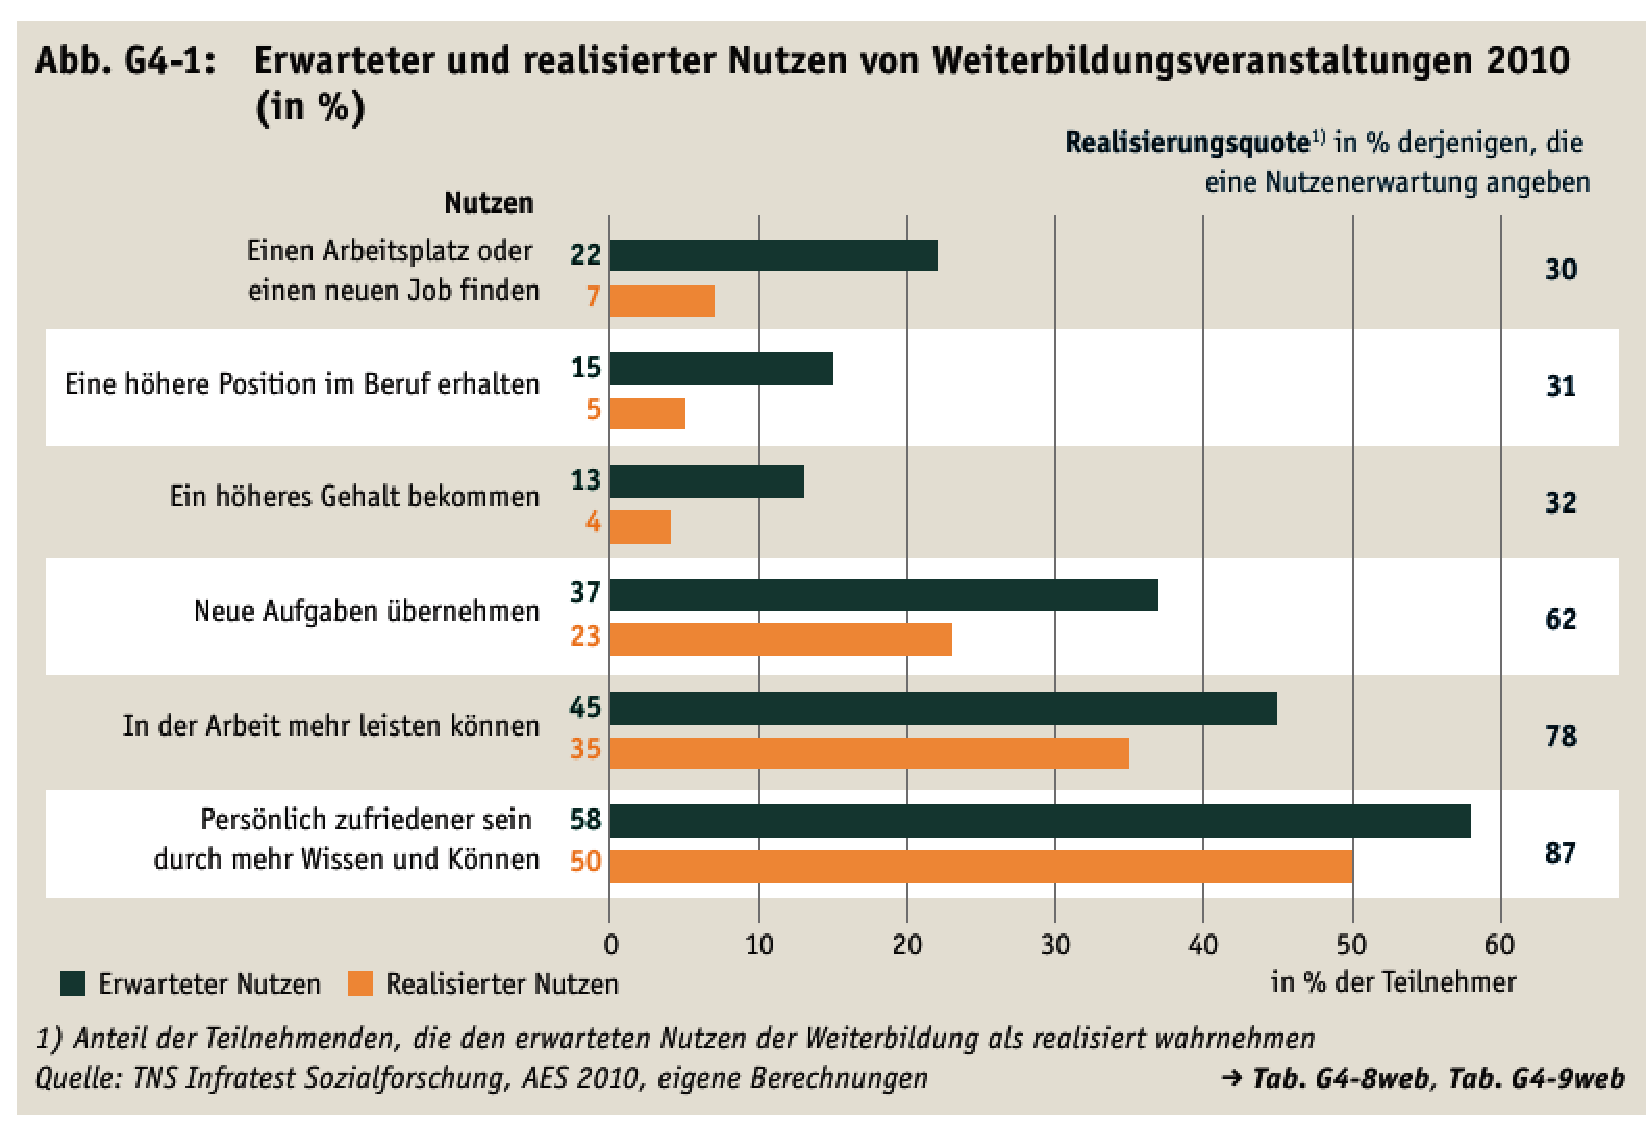
\includegraphics[scale=0.48]{abbg41.pdf}
\caption{Quelle: Bildung in Deutschland 2012, S.153}
\label{}
\end{figure}


Die Studie zeigt außerdem, dass sich mit der erhöhten Zufriedenheit auch die Arbeitsmotivation der Teilnehmer verbessert hat und somit die Leistungsfähigkeit gestiegen ist. Ein gutes Drittel der Teilnehmer konnte nach der beruflichen Weiterbildung mehr leisten als davor. Weitere Veränderungen wurden in den Tätigkeitsbereichen der Arbeitnehmer festgestellt: Knapp ein Viertel der Teilnehmer übernahm nach dem Veranstaltungsbesuch neue Aufgaben
(vgl. "`Lernen bedeutet leben"').

Die Zufriedenheit der Teilnehmer stellt auch in der vorliegenden Studie einen zentralen Qualitätsstandard dar. Sind die Teilnehmenden beispielsweise mit einer Weiterbildungsmaßnahme unzufrieden, so ist es sehr wahrscheinlich, dass diese kein weiteres Mal in Anspruch genommen wird. Die Teilnehmerzufriedenheit zeigt sowohl Schwächen als auch Stärken einer Fortbildung auf und gibt somit wichtige Hinweise, in welchen Bereichen der Fortbildung es eventuell Verbesserungsbedarf besteht. 

Um sowohl Teilnehmern als auch Anbietern mehr Transparenz zu schaffen und ihnen Orientierung zu erleichtern, wurden im Rahmen der Qualitätsdebatte durch eine Expertengruppe mit Vertretern aus Gewerkschaften, Anbietern von Fort- und Weiterbildungen sowie Vertretern aus Wissenschaft und Forschung im Arbeitsfeld Bildung, Betreuung und Erziehung  in Kindertageseinrichtungen einheitliche Standards für die Qualität in der Fort- und Weiterbildung formuliert. Die formulierten Standards in den jeweiligen Qualitätsdimensionen sind für alle Fort- und Weiterbildungsformate relevant. Dazu gehören lang- oder mittelfristige Angebote, eintägige oder mehrtägige Veranstaltungen ebenso wie Seminare. Damit die Komplexität der Aufgaben sowie die Prozesse des Arbeitsfeldes in den Bereichen der Bildung, Betreuung und Erziehung von Kindern erfasst werden können, werden die formulierten Standards nach \textit{Orientierungs-, Struktur-, Prozess- und Ergebnisqualität} differenziert (vgl. Expertengruppe Berufsbegleitende Weiterbildung, S. 14). Diese werden im Folgenden dargestellt. 
 
 \subsection{Standards der Orientierungsqualität}
 
Die Standards der Orientierungsqualität untergliedern sich in fünf wesentliche Punkte. Voraussetzung für gute Qualität ist unter anderem, dass sich (1) \textit{"`die Anbieter von Fort- und Weiterbildung bei den Inhalten und der Durchführung ihrer Veranstaltungen an einschlägigen Theorien und aktuellen Ergebnissen wissenschaftlicher Forschung sowie fachwissenschaftlicher Diskurse orientieren"'} (Expertengruppe Berufsbegleitende Weiterbildungsinitiative, 2011, S. 15). Im Mittelpunkt sollten dabei die Erkenntnisse über Bildungsprozesse von Kindern und Erwachsenen stehen. Fragestellung, Methoden und Ergebnisse unterschiedlicher Forschungszusammenhänge und Disziplinen sollen thematisiert sowie in den Bildungsprozess einbezogen und regelmäßig aktualisiert werden (vgl. Expertengruppe Berufsbegleitende Weiterbildungsinitiative, 2011, S. 15-16). Konsequenzen die aus dem Wissen über kindliche Bildungsprozesse für das professionelle Handeln der pädagogischen Fachkräfte zu ziehen sind, werden in den Angeboten der Fort- und Weiterbildung reflektiert. 

Des Weiteren sollten (2) \textit{"`Bildungsprozesse von den Anbietern der Fort- und Weiterbildung so gestaltet werden, das diese auf den lebensweltlichen und biografischen Erfahrungen, Fähigkeiten und Ressourcen der Teilnehmerinnen und Teilnehmer aufbauen und sich auf deren Fragen und Bedürfnisse beziehen"'} (Expertengruppe Berufsbegleitende Weiterbildungsinitiative, 2011, S. 16). Lerngemeinschaften werden wertgeschätzt und Lernprozesse in soziale Bezüge eingebettet. 

Die Anbieter von Fort- und Weiterbildung sollten (3) \textit{sich außerdem an den beruflichen Erfahrungen der pädagogischen Fachkräfte orientieren und deren berufliche Kompetenzen erweitern} (vgl. Expertengruppe Berufsbegleitende Weiterbildungsinitiative, 2011, S. 16). Berufsbiografische Erfahrungen werden in diesem Zusammenhang als Ressource verstanden und wert\-schät\-zend einbezogen. Alle Akteure der gemeinsamen Bildungsprozesse, das heißt die Teilnehmerinnen und Teilnehmer ebenso wie die Referentinnen und Referenten, sind dabei aufgefordert, ihre pädagogischen Haltungen und die zugrunde liegenden berufsbiografischen Erfahrungen offenzulegen und zur Reflexion zu stellen (vgl. Expertengruppe Berufsbegleitende Weiterbildungsinitiative, 2011, S. 17).

Einen weiteren Punkt (4) \textit{stellt die Partizipation und Übernahme von Verantwortung dar. Diese sind für die Anbieter der Fort- und Weiterbildung grundlegend und werden bei allen Beteiligten gefördert }(vgl. Expertengruppe Berufsbegleitende Weiterbildungsinitiative, 2011, S. 17). Fort- und Weiterbildungen haben das Ziel, Teilnehmerinnen und Teilnehmer an der Weiterentwicklung ihres beruflichen Profils und ihres Arbeitsfeldes zu beteiligen. Dazu zählt, dass sie auch den Prozess der Fort- und Weiterbildung aktiv mitgestalten können. 

Ferner sollten (5) \textit{"`die Anbieter der Fort- und Weiterbildungen eine heterogene Zusammensetzung der Lerngruppen als Voraussetzung für inklusive Bildungsprozesse nutzen"'} (Expertengruppe Berufsbegleitende Weiterbildungsinitiative, 2011, S.17).

 \subsection{Standards der Strukturqualität}
 
Aufgabe der Anbieter von Fort- und Weiterbildung ist es, Qua\-li\-fi\-zie\-rungs\-pro\-zes\-se von pädagogischen Fachkräften so zu konzipieren, dass diese ihre Kompetenzen erweitern. Diese Kompetenzen sollen die Fachkräfte dazu befähigen, die Konzepte ihrer Kindertageseinrichtungen weiterzuentwickeln, Kindern Bildungschancen zu eröffnen sowie deren Bildungsprozesse zu begleiten und zu unterstützen. Folgende Standards der Strukturqualität haben einen hohen Stellenwert. 

Zum einen (1) \textit{ermitteln die Anbieter bei den Trägern von Kindertageseinrichtungen den Bedarf an Fort- und Weiterbildung und orientieren sich dabei an deren Konzepten. Auf der Grundlage der jeweiligen Trägerkonzepte entwickeln sie bedarfsgerechte und abgestimmte Angebote. Gegebenenfalls nehmen die Anbieter auch mit den Teams in den Kindertageseinrichtungen Kontakt auf, und klären deren Fort- und Weiterbildungsbedarf} (vgl. Expertengruppe Berufsbegleitende Weiterbildungsinitiative, 2011, S. 18-19). Dabei werden Ziele und Formate der Fort-und Weiterbildungen zwischen Anbietern und Trägern abgestimmt.

Zum zweiten (2) \textit{informieren die Anbieter  ihren Auftraggeber über den Einsatz ihrer Referentinnen und Referenten sowie über die Bereitstellung angemessener Räume und deren Ausstattung.} Transparenz wird unter anderem dadurch geschaffen, dass Ausschreibungen und Konzepte von Veranstaltungen der Fort- und Weiterbildung nähere Informationen über Inhalte, Ziele, Prozesse und erwartete Ergebnisse enthalten. Kommuniziert werden ebenfalls Angaben über die Auswahl und Kompetenzen der Referentinnen und Referenten sowie Informationen über die Ausstattung der Räumlichkeiten und Fortbildungsmaterialien (vgl. Expertengruppe Berufsbegleitende Weiterbildungsinitiative, 2011, S. 19). 

Einen dritten Standard der Strukturqualität stellt (3) \textit{die regelmäßige Überprüfung der Angebote und Veranstaltungsprogramme durch die Anbieter dar. Die Er\-geb\-nis\-se sollten im jeweiligen Kontext kommuniziert und bei der Weiterentwicklung der Angebote berücksichtigt werden. }Um Transparenz zu schaffen sollten der Verlauf und die Ergebnisse jeder Veranstaltung der Fort-und Weiterbildung in angemessener Weise und mit fundierten Methoden kontrolliert werden. Eingesetzt werden können hierfür sowohl einfache Rück\-kopp\-lungs\-ver\-fahr\-en als auch komplexere Evaluationsinstrumente. Der Anbieter sollte die Rück\-mel\-dung\-en und Reflexionsergebnisse aller Beteiligten für die Ver\-bes\-ser\-ung und Weiterentwicklung der Angebote nutzen (vgl. Expertengruppe Berufsbegleitende Weiterbildungsinitiative, 2011, S. 19-20). 

Den vierten und letzten wesentlichen Standard für die Strukturqualität stellt (4) \textit{die durch strukturelle Maßnahmen gewährleistete Weiterentwicklung der wis\-sen\-schaft\-lich-fach\-lich\-en und der persönlichen Kompetenzen der Referentinnen und Referenten dar. Sichergestellt werden muss, dass die Grund\-sät\-ze der Orientierungsqualität der Anbieter den Referentinnen und Referenten bekannt sind beziehungsweise vermittelt werden.} Die Qualität der Fort- und Weiterbildungen wird durch die Qualifikationen der Referentinnen und Referenten maßgeblich mitbestimmt. Sie repräsentieren und realisieren die grundlegenden Orientierungen und Leitziele des Fort- und Weiterbildungsanbieters und entwickeln diese im Sinne der Partizipation weiter. Daher stellt ein wesentliches Element der Strukturqualität die systematische Förderung der Kompetenzentwicklung der angestellten und freien Mitarbeiterinnen und Mitarbeiter dar. Diese wird sichergestellt durch Fort- und Weiterbildungen, durch kollegialen Austausch, durch Supervision sowie durch die Weitergabe von Information (vgl. Expertengruppe Berufsbegleitende Weiterbildungsinitiative, 2011, S. 20).

 \subsection{Standards der Prozessqualität}

Ein wesentliches Kriterium der Prozessqualität ist die Gestaltung von Bildungsprozessen in gemeinsamer Verantwortung aller Beteiligten. Daraus er\-ge\-ben sich die folgenden fünf Standards für Prozessqualität. 
\textit{Bildungsprozesse sollten (1) von den Referentinnen und Referenten der Weiterbildung dialogisch und gemeinsam mit den Teilnehmerinnen und Teilnehmern auf der Basis gegenseitiger Anerkennung angelegt werden. Neugierde soll so als wichtigste Ressource erhalten bleiben und geweckt werden.} Die Fort- und Weiterbildungen von pädagogischen Fachkräften in Kindertageseinrichtungen beziehen sich immer auf die Elemente \textit{Wissen }und\textit{ Können}, \textit{(Selbst-)Reflexion} und \textit{Haltung} sowie auf die Handlungsfertigkeiten in der Praxis (vgl. Expertengruppe Berufsbegleitende Weiterbildungsinitiative, 2011, S. 21-22). 

Die ganz\-heit\-liche Gestaltung von Bildungsprozessen stellt einen zweiten elementaren Standard der Prozessqualität dar. \textit{Die Referentinnen und Referenten gestalten (2) Bildungsprozesse ganzheitlich. Dabei ist wesentlich, dass Bil\-dungs\-pro\-zes\-se zugleich auf der inhaltlichen Ebene, in der Dynamik der Gruppenprozesse und spezifisch für jede einzelne Person stattfinden.} Wichtig ist außerdem, dass die Referenten/innen einschlägige fachwissenschaftliche Referenztheorien der Erwachsenenbildung kennen (vgl. Expertengruppe Berufsbegleitende Weiterbildungsinitiative, 2011, S. 22). 

Der dritte wichtige Standard der Prozessqualität erfordert, \textit{(3) dass die eingesetzten Veranstaltungsformate sowie Methoden und Verfahren dem "` doppelten Auftrag"' der Fort- und Weiterbildung entsprechen.} Dabei sollte die doppelte Zielperspektive berücksichtigt werden. Einerseits bilden sich die Fachkräfte weiter, andererseits müssen die Inhalte und Formen der Bildungsprozesse die Fachkräfte dazu qualifizieren, ähnlich strukturierte Bildungsprozesse der Kinder begleiten zu können. Sich fortzubilden bedeutet  in diesem Zusammenhang auch, Veränderungen zuzulassen (vgl. Expertengruppe Berufsbegleitende Weiterbildungsinitiative, 2011, S. 22-23). 

Außerdem sollte sichergestellt werden, (4) \textit{dass ein breites Set von Methoden, Lernformen und Lernverhalten, wie das Selbstlernen, Coaching, Seminare und Lernwerkstätten bereitgestellt werden. Teilnehmer/innen sollen so befähigt werden, ihre Lernerfahrungen an das Team weiterzuvermitteln und als Multiplikatoren fungieren. Durch eine enge Verzahnung von Wissensvermittlung, Praxiserprobung, Reflexion und erneuter Wissensvermittlung gehört der Transfer in die Praxis zur Struktur des Angebots} (vgl. Expertengruppe Berufsbegleitende Weiterbildungsinitiative, 2011, S. 23). 

Den fünften und letzten elementaren Standard für die Prozessqualität stellt (5)\textit{ die Verantwortlichkeit der Referenten/innen dar, den gemeinsamen sowie individuellen Bildungsprozess unter Mitwirkung aller Beteiligten angemessen zu gestalten und zu visualisieren.} Darunter ist unter anderem zu verstehen, dass Lernprozesse nachvollziehbar, transparent und unter Beteiligung aller Teilnehmer gestaltet werden. Diese Prozesse zu reflektieren, zu visualisieren und in geeigneter Form zu dokumentieren, führt dazu, dass Bildungsprozesse in ihrer Komplexität sichtbar, Inhalte festgehalten, Gruppenprozesse nachvollzogen und individuelle Bildungsprozesse in ihrer Subjektivität dargestellt werden (vgl. Expertengruppe Berufsbegleitende Weiterbildungsinitiative, 2011, S. 24). 

 \subsection{Standards der Ergebnisqualität}
 
Ein Nachweis über die angestrebten positiven Wirkungen von Fort- und Weiterbildungen ist ein berechtigtes Anliegen aller Beteiligten – insbesondere auch der Träger von Kindertageseinrichtungen. Gerade deswegen hat auch die Ergebnisqualität einen hohen Stellenwert. Die Ergebnisqualität beschreibt die fort- und weiterbildungsbezogenen Resultate und Wirkungen seitens der Teilnehmerinnen und Teilnehmer von Fort- und Weiterbildungen. Voraussetzung für die Überprüfung der Ergebnisqualität sind deshalb nachvollziehbare Weiterbildungsziele. Folgende drei Standards sind für die Ergebnisqualität relevant (vgl. Expertengruppe Berufsbegleitende Weiterbildungsinitiative,\linebreak 2011, S. 25). 

Zum ersten sind (1) \textit{die angestrebten Ziele und Ergebnisse der Fort- und Weiterbildungen verbindliche Vorgaben für das Handeln der Referentinnen und Referenten. }Den Referentinnen und Referenten kommt daher eine wichtige Vorbildfunktion zu. Ihre Fachlichkeit, ihr Handeln und vor allem ihre Dialogfähigkeit korrespondieren mit den Möglichkeiten, bestimmte Ziele zu erreichen (vgl. Expertengruppe Berufsbegleitende Weiterbildungsinitiative, 2011, S. 25). 

Den zweiten wichtigen Standard stellen (2) \textit{die Reflexion des eigenen Handels sowie die Möglichkeiten und Grenzen einer Realisierung der angestrebten Ziele durch die Referenten/innen dar}. Dazu gehört die kritische Auseinandersetzung mit dem Verlauf der Fortbildungsveranstaltung sowie den Rückmeldungen der Teilnehmer/-innen. Dokumentationen über den Verlauf und über die Rückmeldungen der Fort- und Weiterbildungen sind für den Träger von Kindertageseinrichtungen eine wichtige und unverzichtbare Informationsquelle, aus der hervorgeht, welche Bildungsprozesse angestoßen wurden und inwieweit die vereinbarten Ziele erreicht werden konnten (vgl. Expertengruppe Berufsbegleitende Weiterbildungsinitiative, 2011, S. 26). 

\textit{Die Dokumentation und Evaluation der Ergebnisse der Fortbildung bilden (3) den letzten elementaren Standard der Ergebnisqualität}. Ein grundlegendes Kriterium der Ergebnisqualität ist die Reflexion des Wei\-ter\-bil\-dungs\-pro\-zes\-ses durch alle Beteiligten. So wird ermöglicht, Konsequenzen für die Organisation sowie Gestaltung zukünftiger Weiterbildungsveranstaltungen zu ziehen. Ein fachlich aufwendiges aber nicht zu vernachlässigendes Verfahren ist die nach Ablauf der Veranstaltung durchzuführende Evaluation der Wirkung der Fort-und Weiterbildung im Praxisfeld. Mit diesem Verfahren kann die Nachhaltigkeit von Fort-und Weiterbildungen am ehesten festgestellt werden (vgl. Expertengruppe Berufsbegleitende Weiterbildungsinitiative, 2011, S. 26). 

	Die oben formulierten Qualitätsstandards stellen ein wichtiges Kriterium für die Beurteilung der Qualität von Fort- und Weiterbildungsmaßnahmen pädagogischer Fachkräfte dar. Sie bilden nicht nur ein wichtiges Orientierungskriterium für bereits bestehende Wei\-ter\-bil\-dungs\-kon\-zep\-te, sondern dienen auch als wichtige Leitorientierungen bei der Entwicklung neuer Weiterbildungskonzepte. 
	
	Im folgenden Kapitel wird zunächst das Fortbildungsprogramm \textit{"`Qualität von Anfang an"'} dargestellt. Im späteren Verlauf des Forschungsberichts wird unter anderem untersucht, inwieweit das Programm den zuvor formulierten Qualitätsstandards entspricht bzw. welche dieses erfüllt.
 
 \section{Qualifizierungsprogramm zur Betreuung, \\Bildung und Erziehung von Kindern unter  drei Jahren \textit{"`Qualität von Anfang an"'}}
 
Wie bereits erwähnt wurde, führen einerseits die Einführung der Krippenbetreuung und des Rechtsanspruchs auf einen Krippenplatz, andererseits die Notwendigkeit des Einbezugs der aktuellen entwicklungspsychologischen Erkenntnisse in die pädagogische Praxi dazu, dass sich neue Herausforderungen an das frühpädagogische Fachpersonal stellen. Neben der Diskussion der gestiegenen Anforderungen an die frühpädagogischen Fachkräfte in Einrichtungen des Elementarbereichs wurde auch die Debatte um eine qualitativ hochwertige pädagogische Arbeit neu entfacht. Eine gute und qualitativ hochwertige pädagogische Arbeit ist laut Prof. Dr. Wolfgang Tietze für die Entwicklung des Kindes von elementarer Bedeutung und in Kindertageseinrichtungen unabdingbar (vgl. Tietze, et al., 1998, S. 337). Die Qualifikationen der pädagogischen Fachkräfte haben demnach einen bedeutenden Einfluss auf die pädagogische Qualität innerhalb einer Einrichtung. 

	Im Rahmen dieser gestiegenen Anforderungen an gute pädagogische Qualität in Einrichtungen des Elementarbereichs haben sich zahlreiche Fort-und Weiterbildungsangebote auf dem frühpädagogischen Weiterbildungsmarkt etabliert. Eines dieser Angebote ist das Fortbildungs- und Qualifizierungsprogramm zur Betreuung, Bildung und Erziehung unter dreijähriger Kinder \textit{"`Qualität von Anfang an"'} (Lasson \& Grenner, 2008, S. 45). Dieses wurde von PädQUIS, einem Kooperationsinstitut der Freien Universität Berlin, entwickelt. Im Folgenden wird das Programm "`Qualität von Anfang an"' exemplarisch vorgestellt.\\

Das Programm \textit{"`Qualität von Anfang an"'}\\

Das Qualifizierungsprogramm \textit{"`Qualität von Anfang an"'} soll Einrichtungen auf dem Weg begleiten und sie dabei unterstützen, die Angebote für unter drei jährige Kinder zu sichern und zu verbessern. Dabei richtet sich das Qualifizierungsprogramm an Fach- und Leitungskräfte aus Kindertageseinrichtungen, die ihr Angebot für Kinder unter drei Jahren öffnen wollen oder diese bereits betreuen. Die Kompetenzen der pädagogischen Fachkräfte werden in Bezug auf individuelle Kommunikation und Beziehungsgestaltung mit dem Kind bei der entwicklungsbegleitenden ganzheitlichen Förderung sowie in der Gestaltung der Erziehungspartnerschaft mit den Familien reflektiert und erweitert. Leitungskräfte, pädagogische Fachkräfte und Teams erhalten eine unmittelbare und praxisbegleitende Unterstützung und Hilfe, den Bildungsauftrag für jüngere Kinder umzusetzen und in der alltäglichen pädagogischen Arbeit lebendig zu gestalten. Auf diese Weise werden konkrete Impulse für Veränderungen gegeben und die qualitätsorientierte Entwicklung in den Einrichtungen begleitet (vgl. Lasson \& Grenner, 2008, S. 47). Auf der Basis wissenschaftlicher Erkenntnisse aus der Kleinkindpädagogik und Entwicklungspsychologie sowie auf der Grundlage bester Fachpraxis des Nationalen Kriterienkatalogs werden zentrale Themen pädagogischer Qualität bearbeitet und auf die Altersgruppe der unter Dreijährigen mit ihren Besonderheiten im KiTa-Alltag angewandt. Im Zentrum des Fortbildungsprogramms \textit{"`Qualität von Anfang an"'} stehen folgende Qualitätsbereiche, die zentrale Themen- und Schlüsselaufgaben für Kindertageseinrichtungen darstellen:\\

\textit{Soziale und emotionale Entwicklung}\\
Gegenstand dieses Themenkomplexes ist die Vermittlung eines umfassenden Überblicks über entwicklungspsychologische Grundlagen sozial-emotionaler Entwicklung.\\

\textit{Bindung und Eingewöhnung}\\
Zentrale Aspekte im Themenkomplex "`Bindung und Eingewöhnung"' ist eine umfassende Einführung in die Bindungstheorie sowie die Bedeutung von Bindungsbeziehung der unter dreijährigen Kinder. Ein weiterer Schwerpunkt liegt auf der Thematik der Kooperation mit Eltern und Familie. Darüber hinaus spielt die Bindungstheorie bei der Eingewöhnung eine wichtige Rolle bei der Erarbeitung des Themenkomplexes.\\

\textit{Wahrnehmung, Bewegung und Sprache }\\
Vermittelt wird ein ganzheitliches Verständnis von Sprachentwicklung und Bewegung. Es werden sowohl Aspekte der motorischen, kognitiven, sprachlichen als auch der sozial-emotionalen Entwicklung behandelt.\\

\textit{Spiel}\\
Teilnehmer/-innen erhalten einen Einblick in spieltheoretische Grundlagen. Vermittelt wird dabei ein umfassender Überblick über die Bedeutung des Spiels und den Zusammenhang für die kindliche Entwicklung in allen Entwicklungsbereichen.\\

\textit{Beobachtung, Dokumentation und Planung}\\
Der Themenkomplex thematisiert die Bedeutung regelmäßiger und entwicklungsbegleitender Beobachtung. Dabei werden verschiedene Beo\-bach\-tungs\-möglich\-kei\-ten vorgestellt.\\

\textit{Beziehungsorientierte Pflege}\\
Vermittelt werden hier zentrale Aspekte bester Fachpraxis in den Qua\-li\-täts\-be\-rei\-chen "`Mahlzeiten und Ernährung"', "`Ruhe und Schlafen"' sowie "`Gesundheit und Körperpflege"'. Dabei werden fachtheoretische und fachpraktische Kenntnisse in der Pflege unter dreijähriger Kinder erarbeitet.\\

\textit{Gestaltung von Räumen, Materialangebot und Sicherheit}\\
Fortbildungsteilnehmern/-innen wird vermittelt, welche Bedürfnisse Kin\-der unter drei Jahren hinsichtlich der Raumgestaltung in Kindertageseinrichtungen haben und welche Gesichtspunkte beachtet werden sollen. Einen weiteren Schwerpunkt stellt das Thema "`Sicherheit"' dar.\\

\textit{Kindgerechte Tagesgestaltung}\\
Teilnehmer/-innen erhalten in diesem Qualitätsbereich einen ausführlichen Überblick über die Tagesgestaltung in Kindertageseinrichtungen. Hervorgehoben werden hierbei die Thematiken der Partizipation sowie der individuelle Rhythmus von Kindern in den ersten drei Lebensjahren (vgl. PädQUIS U3-Rahmenkonzeption, 2010, S.5-8)\\

\textit{Zusammenarbeit mit Familien}\\
Vermittelt werden wichtige Aspekte der Zusammenarbeit mit Eltern bzw. Familien. Im Fokus steht dabei das gemeinsame Bemühen um die Entwicklung und das Wohlbefinden der Kinder (vgl. Dittrich, Grenner, Groot-Wilken, Sommerfeld \& Hanisch, 2007, S. 233). 

Die Fortbildung erstreckt sich über einen Zeitraum von ca. 12 Monaten. In diesem Zeitabschnitt finden zehn Kurstermine statt. Zwischen den einzelnen Kursterminen liegt jeweils eine etwa vier- bis sechswöchige Praxisphase, in der die Teilnehmer/innen vorbereitete Praxisanregungen umsetzen können. Auf diese Weise soll ein Transfer der Kursinhalte in die Einrichtungen ermöglicht  werden. Unterstützt wird dieser Transfer durch verschiedene von PädQUIS gestellte Arbeitsmaterialien mit kompakten Informationen zu den Qualitätsbereichen.  
Folgende Arbeitsmaterialien werden von PädQUIS bereitgestellt:

\begin{itemize}

\item Praxisnahe und aktuelle Fachliteratur und Informationen
\item Instrumente zur Selbstevaluation für alle Themen und Bereiche
\item Unterstützende Anschauungs- und Arbeitsmaterialien 
\item Instrumente zur Beobachtung und Dokumentation
\end{itemize}

Die Fortbildung wird von einer durch PädQUIS geschulten Mitarbeiter/-in geleitet und methodisch vielfältig und abwechslungsreich gestaltet. Dazu gehören unter anderem Impulsreferate, Präsentationen, angeleitete Reflexion und Erfahrungsaustausch, Film- und Medienbeiträge sowie Methoden der Gruppen- und Teamarbeit.
Als Nachweis über die Teilnahme am Programm sowie über die vermittelten Inhalte des Kurses erhalten die Teilnehmer/-innen mit Abschluss des Kurses ein Zertifikat. Darüber hinaus können die Teilnehmer/-innen ein Einrichtungs-Zertifikat erwerben. Erworben werden kann dies über eine schriftliche Dokumentation beziehungsweise Darstellung der individuellen Veränderungen und Umsetzungsschritte in der Einrichtung (vgl. Lasson \& Grenner, 2008, S. 48).

Im folgenden Kapitel folgt die empirische Analyse des Programms \textit{"`Qua\-li\-tät von Anfang an"'.} Die Fragestellung und Hypothesen werden formuliert und die Daten anschließend mit geeigneten statistischen Verfahren untersucht. Die daraus folgenden Ergebnisse werden im darauf folgenden Abschnitt vorgestellt.
\pagebreak
\section{Empirische Analyse des Programms\\ "`Qua\-li\-tät von Anfang an"'}
\subsection{Fragestellung und Hypothesen}

Aus den dargestellten theoretischen Ausführungen lässt sich die Fragestellung des vorliegenden Forschungsberichtes konkretisieren:\\

\textit{Wodurch zeichnet sich gute Qualität im Programm zur Betreuung, Bildung und Erziehung von Kindern unter drei Jahren \textit{"`Qualität von Anfang an"'} aus und durch welche Faktoren wird sie beeinflusst und bestimmt?}\\

Im Zentrum der Untersuchung steht die Analyse des Programms\textit{ "`Qualität von Anfang an"'}. Dabei soll überprüft werden, ob die zuvor durch die Experten formulierten Qualitätsstandards wie Teilnehmerzufriedenheit, Praxisorientierung der Inhalte sowie die Qualifizierung des Kursleiters erfüllt werden. Herausgearbeitet wird hier unter anderem, welcher Zusammenhang zwischen Kursleitererfahrung und Teilnehmerzufriedenheit besteht.

Auf Grund der theoretischen Erläuterungen lassen sich folgende konkrete Hypothesen für die empirische Untersuchung aufstellen, die anhand der vorliegenden Daten geprüft werden sollen:


\begin{enumerate}
\itshape
\item Je mehr Erfahrung die Referent/-innen als Kursleiter/-innen haben, desto besser fällt die Beurteilung des Kurses durch die Teilnehmer/-innen aus.

\item Je besser die Bewertung der Gestaltung des Tages, desto besser die Bewertung des Arbeitskreises insgesamt.

\item Je besser die Bewertung der Präsentation der Inhalte durch den Kursleiter, desto besser die Bewertung des Arbeitskreises insgesamt.

\item Je besser die Bewertung der Arbeitsform und Methoden, desto besser die Bewertung des Arbeitskreises insgesamt.

\item Je besser die Bewertung der Nutzbarkeit der Inhalte für den eigenen Arbeitsbereich, desto besser die Bewertung des Arbeitskreises insgesamt.

\item Je besser die Bewertung der Arbeitsatmosphäre, desto besser die Bewertung des Arbeitskreises insgesamt.

\item Die Bewertungen der Kursleiter/-innen durch die Teilnehmer/-innen bezüglich der Arbeitsform, Arbeitsatmosphäre sowie des fachlichen Austauschs unterscheiden sich untereinander.
\end{enumerate}

\normalfont

\subsection{Methodische Vorgehensweisen}
\subsubsection{Datengrundlage}

Wie bereits in der Einleitung ausgeführt wurde, geht es in der vorliegenden Arbeit um die Fort- und Weiterbildungslandschaft frühpädagogischer Fachkräfte. Im Mittelpunkt der empirischen Auseinandersetzung steht spe\-zi\-ell die Analyse des Programms \textit{"`Qualität von Anfang an"'}. In der ersten Linie soll die Zufriedenheit der Teilnehmer/-innen mit dem Programm untersucht werden. Zusätzlich beschäftigen wir uns mit der Frage, welche durch die Experten entwickelten Qualitätsstandards für die Fort- und Weiterbildungsangebote das Programm erfüllt. 

Insgesamt lagen uns Daten von 2861 Fragebögen vor. Davon konnten 1018 standardisierte und anonymisierte Teilnehmerfragebögen aus sechs verschiedenen Kursen des Programms \textit{"`Qualität von Anfang an"'} sowie fünf Kursleiterfragebögen in der empirischen Analyse der vorliegenden Studie berücksichtigt werden. Die Felduntersuchung war querschnittlich angelegt und wurde anhand schriftlicher Befragung über einen Zeitraum von 5 Jahren (2007-2012) durchgeführt. Die Daten wurden mittels einer Vollerhebung erhoben. Die Teilnehmer/-innen erhielten nach jedem Arbeitskreis von jeweiligen Kursleiter/-innen einen Fragebogen zum Ausfüllen. Nach dem Beantworten der Fragen wurden die Feedbackbögen eingesammelt und postalisch an das PädQUIS-Institut zurückgesendet. 

Um  auch die Kursleiterinformationen zu erhalten, wurden die Kursleiter/-innen per E-mail über unser Vorhaben informiert und gebeten, an dem Projekt teilzunehmen. Im Anschluss erhielten die Kursleiter/-innen einen Fragebogen, welcher per E-Mail an sie gesendet wurde. Die Rücksendung der Fragebögen erfolgte sowohl per E-Mail als auch postalisch.

\subsubsection{Beschreibung der Stichprobe}

Insgesamt umfasst die Untersuchung die Daten von N=7 Kursleiter/-innen, die an dem PädQUIS-Institut als freie Mitarbeiter/-innen tätig sind bzw. tätig waren. Des Weiteren enthält der Datensatz 2861 Fälle. Die Kurse bestehen im Durchschnitt aus 20-25 Teilnehmer/-innen. Das heißt, in der vorliegenden Untersuchung haben ca. 120-150 Personen teilgenommen. Die Differenz in der Anzahl der von den Kursleiter/-innen durchgeführten Kurse führte folglich zu einer sehr unterschiedlichen Verteilung der Daten. Um statistisch relevante Aussagen treffen zu können, musste eine Auswahl der Fälle aus dem vorliegenden Datensatz getroffen werden. Nach der Reduktion der Daten flossen letztlich 1018 Feedbackbögen von sechs zuletzt abgeschlossenen Kursen jeweils eines Kursleiters/einer Kursleiterin sowie die Daten von sechs Referenten/-innen (1=männlich, 5=weiblich) in die statistische Analyse ein. Aufgrund einer geringen Rücklaufquote konnten die Daten eines Kursleiters nicht berücksichtigt werden. 

Durch das Anonymisieren der Fragebögen liegen zu den Teilnehmer/-innen keine persönlichen Angaben vor. Zu den Kursleiter/-innen des Fortbildungsprogramms konnten jedoch persönliche Daten erhoben werden. Beispielsweise besitzen alle Kursleiter/-innen eine abgeschlossene Schulausbildung (Hochschulreife und Fachhochschulreife) so\-wie einen pädagogischen Berufsabschluss. Bis auf eine/n Kursleiter/-in, der/die sich derzeit noch im Studium befindet, verfügen alle Kursleiter/-innen über einen Fachhochschulabschluss oder einen Hochschulabschluss. 

Die Al\-ters\-ver\-teil\-ung ist durch folgende Parameter beschrieben: das arithmetische Mittel des Alters beträgt $\bar x= 41,8$ und Median= 36, bei einer Standardabweichung s=10.25, Minimum 31 Jahre, Maximum 62 Jahre. Entsprechend breit ist auch die Berufserfahrung der Befragten als Kursleiter/-in. Dabei erstrecken sich die Angaben von einem Jahr bis zu 36 Jahren Berufserfahrung. Als U3 Kursleiter/-in bei PädQUIS umfasst die Berufserfahrung der befragten Kursleiter/-innen ein bis fünf Jahre. Die meisten Kursleiter/-innen verfügen über eine zusätzliche Ausbildung bzw. Weiterbildung zu Fortbildner/-in.

\subsubsection{Instrumente}

Im Folgenden werden die für Erhebung verwendeten Instrumente vorgestellt. Wie bereits erwähnt, wurden die Teilnehmer/-innen des Programms \textit{"`Qualität von Anfang an"'} ebenso wie die Kursleiter/-innen, die am PädQUIS-Institut tätig sind bzw. waren, befragt. Im Vordergrund der schriftlichen Befragung stand die Einschätzung der Zufriedenheit von Teilnehmer/-innen mit dem Programm \textit{"`Qualität von Anfang an"'}. Der Teilnehmerfragebogen wurde von wissenschaftlichen Mitarbeiter/-innen des PädQUIS-Instituts entwickelt. Er ist in neun geschlossene und vier offene Fragen  gegliedert (siehe Anhang A 8. Teilnehmerfragebogen).
Anhand des Fragebogens konnten die Teilnehmer/-innen die Materialien und Unterlagen, die Nutzbarkeit der Inhalte für den eigenen Arbeitsbereich, Arbeitsformen und Methoden des Kursleiters, die Gestaltung des Tages und die Präsentation der Inhalte durch den Kursleiter, das Eingehen des Kursleiters auf die Fragen der Teilnehmer/-innen sowie die Arbeitsatmosphäre und die Möglichkeit zum fachlichen Austausch mit Kollegen bewerten. Die geschlossenen Fragen konnten auf einer fünfstufigen Werteskala (5="'sehr gut"', 4="'gut"', 3="'teilweise gut"', 2="'weniger gut"' und 1="'gar nicht gut"') beantwortet werden. Neben den geschlossenen Fragen wurden die Teilnehmer/-innen gebeten, zu vier offen formulierten Fragen Stellung zu beziehen. Eine dieser Fragen lautete beispielsweise: \textit{"`Gut gefallen hat mir heute: ..."'} oder \textit{"`Nicht gefallen hat mir heute:…"'} Die offenen Fragestellungen wurden in den Fragebogen aufgenommen, um einen Abgleich zwischen den statistischen Werten und der persönlichen Einschätzung der frühpädagogischen Fachkräfte herzustellen. So lassen sich unter anderem Rückschlüsse auf Stärken und Schwächen des Qualifizierungsprogramms schließen. Dies kann wiederum zur Qualitätsoptimierung genutzt werden.

Der Kursleiterfragebogen wurde von Iryna Karpyuk und Sarah Amelie Schroeder, studentischen Mitarbeiterinnen von PädQUIS, erstellt. Ziel des eingesetzten Fragebogens war die Erfragung allgemeiner Kursleiterinformationen, um diese in die spätere statistische Analyse einfließen zu lassen. Eventuelle Zusammenhänge zwischen beruflicher Erfahrungsdauer und der Bewertung durch die Teilnehmer/-innen konnten auf diese Weise erarbeitet werden. Der Kursleiterfragebogen beinhaltete ebenfalls geschlossene (4) und offene (3) Fragen. Erhoben wurden zum Beispiel Informationen zum Bildungsstand, zu Kursleitererfahrungen, zur aktuellen Tätigkeit, zu fachspezifischen Weiterbildungen der Kursleiter/-innen etc. Der Fragebogen ist dem Anhang A 7. Kursleiterfragebogen beigefügt.


\subsection{Ergebnisse}

Im ersten Schritt werden die Daten mittels deskriptiver Maße wie zum Beispiel arithmetisches Mittel, Median, Standardabweichung, Häufigkeiten etc. dar\-ge\-stellt. Zur Überprüfung der formulierten Hypothesen werden zunächst Korrelationsanalysen durchgeführt. Die Ergebnisse der Korrelationsanalyse sind dem Anhang beigefügt. Dadurch sollen erste Erkenntnisse über die Zusammenhänge der abhängigen und unabhängigen Variablen gewonnen werden. Um genauere Aussagen über die Gültigkeit der Hypothesen treffen zu können, werden im Anschluss eine Faktorenanalyse, eine multiple Regression sowie multivariate Varianzanalysen durchgeführt. Die Auswertung der Daten erfolgt mittels der Statistiksoftware SPSS. Mit Hilfe dieser Ergebnisse kann man schließlich die aufgestellten Hypothesen verifizieren bzw. widerlegen. Das theoretische Analyseverfahren der oben genannten Methoden wird im folgenden Abschnitt vorgestellt. 

Im vorliegenden Bericht richtet sich unser Hauptaugenmerk auf die Untersuchung der Zufriedenheit der Teilnehmer/-innen mit dem Programm \textit{"`Qualität von Anfang an"'}. Die folgende Tabelle stellt die deskriptiven Ergebnisse der durchgeführten Analyse vor. 

\subsubsection{Deskriptive Ergebnisse}

In der unten stehenden Tabelle werden die deskriptiven Statistiken dargestellt. Aus der Tabelle geht hervor, dass die Teilnehmer/-innen insgesamt mit den besuchten Kursen zufrieden sind. Die Bewertung liegt im Durchschnitt im Bereich von "`gut"' bis "`sehr gut"'. Am besten hat das Bewertungsitem \textit{"`das Eingehen des Kursleiters auf die Fragen der Teilnehmer"'} abgeschnitten. Der Mittelwert für dieses Item liegt bei $\bar x$= 4,53 mit einer Standardabweichung von .58., gefolgt vom Item \textit{"`die Bewertung der Materialien und Unterlagen"'} mit einem Mittelwert von $\bar x$= 4,48 und einer Standardabweichung .55. Den niedrigsten Mittelwert mit $\bar x$= 4,18 weist das Bewertungsitem \textit{"`die Mög\-lich\-keit zum fachlichen Austausch mit Kollegen"'} auf. Im Vergleich zu anderen bewerteten Aspekten liegt hier eine höhere Streuung vor. Insgesamt unterscheiden sich die Mittelwerte der Items jedoch nur marginal voneinander. 

\begin{table}[!ht]
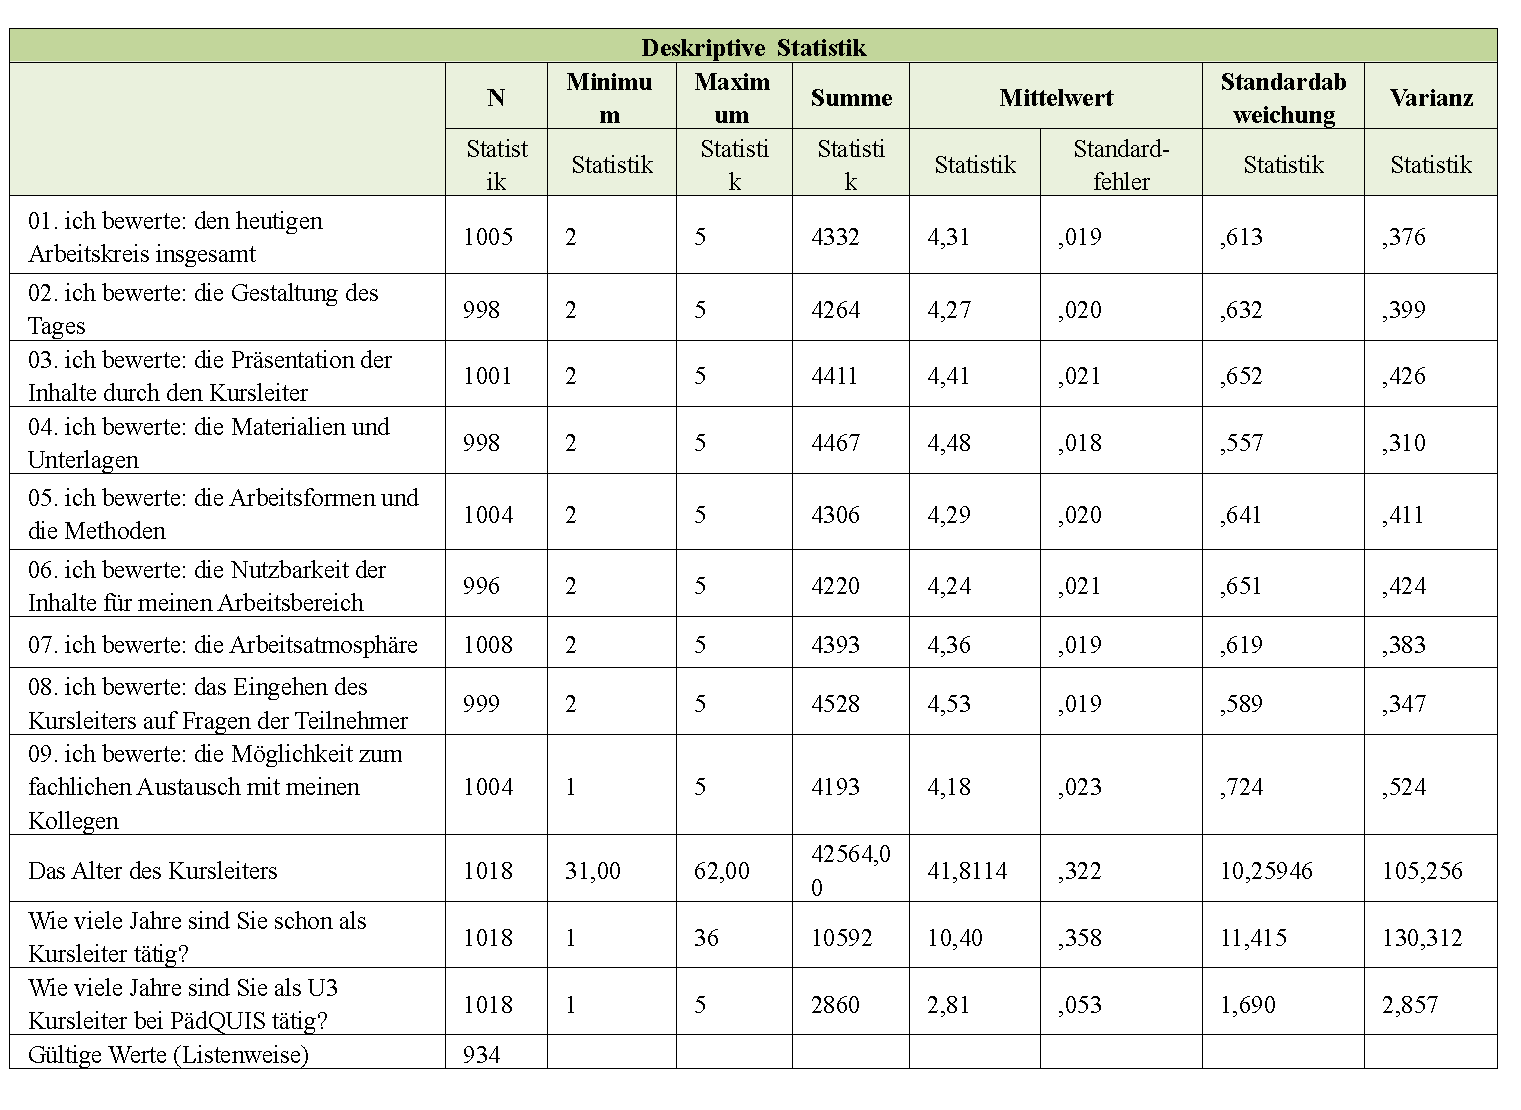
\includegraphics[scale=0.54]{tab05.pdf}
\caption{Deskriptive Statistik}
\label{}
\end{table}


Die Auswertungsergebnisse zeigen, dass die Teilnehmenden das Fortbildungsprogramm \textit{"`Qualität von Anfang an"'} insgesamt mit "`sehr zufrieden"' bis "`zufrieden"' bewerteten. Weiterhin hat die Analyse ergeben, dass der fachlich-kollegiale Austausch sowie die Praxisnähe des Kurses eine wesentliche Rolle für die Zufriedenheit mit dem Kurs spielen. 

\begin{table}[!ht]
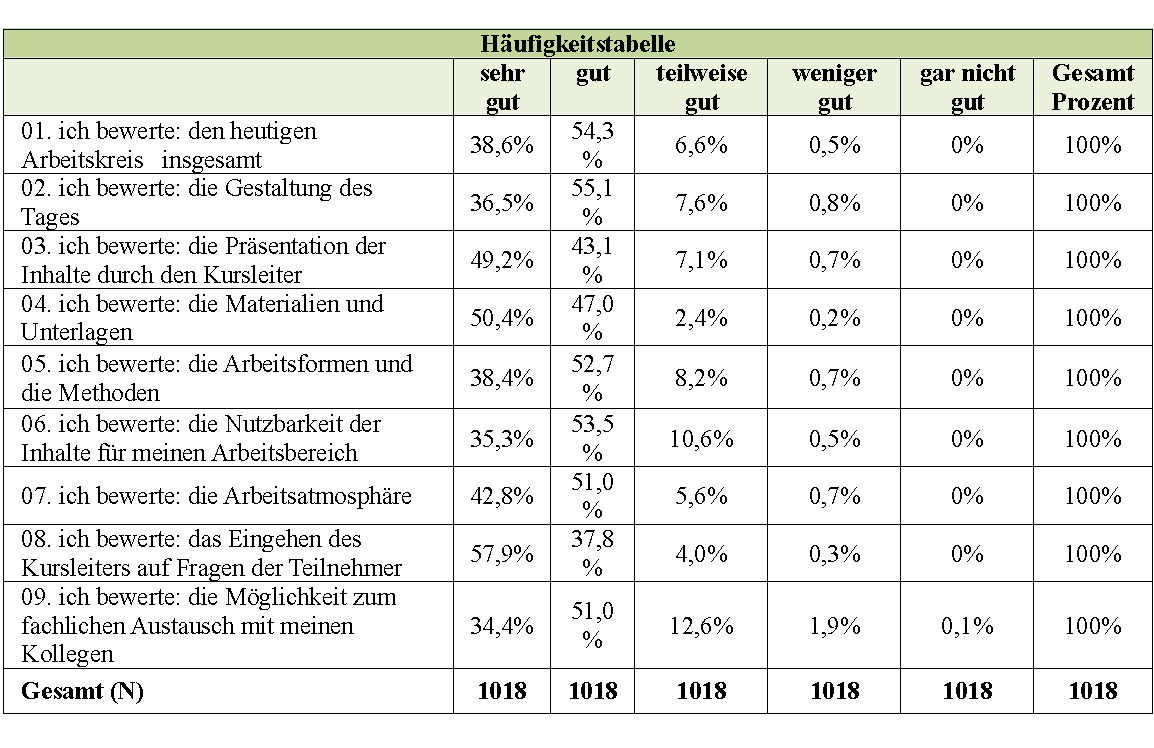
\includegraphics[scale=0.7]{tab06.pdf}
\caption{Häufigkeiten}
\label{}
\end{table}

Mit der Möglichkeit zum fachlichen Austausch mit den Kollegen waren 34,4\% der Teilnehmer/-innen "`sehr zufrieden"' und 51\% "`zufrieden"'. 14,6\% der Befragten meldeten Kritik zu diesem Aspekt an und bewerteten das Item mit "`teilweise"' bis "`gar nicht gut"'.

Die Vermittlung praxisorientierter Inhalte wird in der Forschung als ein wesentlicher Aspekt für die gute Qualität genannt. Das heißt, dass es für die Teilnehmenden sehr wichtig ist, dass die Inhalte des Kurses in die Praxis übertragbar und umsetzbar sind. In diesem Fall wurde die Nutzbarkeit der Inhalte für den eigenen Arbeitsbereich von 35\% der Befragten mit "`sehr gut"' und 53,5\% als "`gut"' bewertet. 11,1\% haben "`teilweise"' bzw. "`weniger gut"' angekreuzt. 

95,7\% sind mit dem Eingehen des Kursleiters auf die Fragen der Teilnehmer zufrieden. Nur 4,3\% äußerten Kritik zu diesem Aspekt und bewerten das Item also mit "`teilweise"' bis "`weniger gut"'. 

Die Arbeitsatmosphäre haben 93,8\% der Teilnehmer/-innen als "`sehr gut"' bis "`gut"' eingeschätzt und 6,3\% bewerten dieses mit "`teilweise"' bis "`weniger gut"'. 

Die Arbeitsformen und Methoden, die bei verschiedenen Fort- und Weiterbildungen zur Anwendung kommen, sind mittlerweile sehr umfangreich und vielfältig. Da diese einen großen Einfluss auf die Wahl des Fortbildungsprogramms haben können, wurde auch hier geschaut, ob die Teilnehmer/-innen mit den Arbeitsformen und Methoden des Programms \textit{"`Qualität von Anfang an"'} zufrieden sind. Die Ergebnisse haben gezeigt, dass 91,1\% "`zufrieden"' und 8,9\% der Befragten nur "`teilweise"' bzw. "`weniger zufrieden"' sind. 

Mit Materialien und Unterlagen waren 97,4\% der Teilnehmer/-innen "`zufrieden"' und lediglich 2,6\% "`teilweise"' bzw. "`weniger zufrieden"'. 

Präsentation der Inhalte durch den Kursleiter wurde mit 49,2\% als "`sehr gut"', 43,1\% als "`gut"' und 7,8\% als "`teilweise gut"' bzw. "`weniger gut"' eingeschätzt. 

Die Gestaltung des Tages haben 91,6\% mit "`gut"' bis "`sehr gut"' und 8,4\% mit "`teilweise gut"' bis "`weniger gut"' bewertet. 92,9\% waren insgesamt mit dem jeweiligen Arbeitskreis zufrieden und nur 7,1\% der pädagogischen Fachkräfte waren "`teilweise"' bzw. "`weniger zufrieden"'.

\subsubsection{Faktorenanalyse}

Die Faktorenanalyse ist ein Verfahren, welches es ermöglicht, eine größere Anzahl von Variablen auf eine kleinere Anzahl zu reduzieren. Dabei wird eine Vielzahl von Variablen, von denen nicht bekannt ist, ob und in welcher Weise sie etwas miteinander gemeinsam haben, in Gruppen aufgeteilt und zu einem Faktor zusammengefasst. Ziel der Faktorenanalyse ist es also, solche Faktoren zu ermitteln, welche die beobachteten Zusammenhänge zwischen den gegebenen Variablen möglichst vollständig erklären. Es wird zwischen der explorativen und konfirmatorischen Faktorenanalyse unterschieden. Bei der explorativen Analyse ist von vornherein nicht bekannt, ob und in welcher Weise die in die Faktorenanalyse eingehenden Variablen miteinander zusammenhängen. Ein Zusammenhang wird lediglich vermutet. Der konfirmatorischen Faktorenanalyse liegt bereits von Anfang an ein Modell möglicher hypothetischer Faktoren zugrunde (vgl. Bühl, 2006, S.485-486). 

Da vor der Durchführung der  vorliegenden Untersuchung lediglich bestimmte Zusammenhänge vermutet wurden, wurde hier eine explorative Faktorenanalyse durchgeführt. 

Im ersten Schritt der Faktorenanalyse wurde untersucht, wie die Struktur der Daten ist und in welcher Weise sich Faktoren bilden. Die Korrelationsanalyse (siehe Anhang A 2. Korrelationsanalyse)
hat gezeigt, dass alle Items sehr hoch miteinander korrelieren und sich somit gut für eine Faktorenanalyse eignen. Auch \textit{der KMO-Index (.904)} und \textit{der Barlett-Test (Sig. .000)} zeigen, dass zwischen allen Variablen ein nennenswerter Zusammenhang besteht. Zwar hat die durchgeführte Faktorenanalyse eine Ein-Faktorenstruktur ergeben: das heißt, dass alle von den Teilnehmenden bewerteten Items auf einem Faktor luden. Dadurch jedoch, dass sich die Items inhaltlich voneinander unterschieden, wurde in der Analyse ermittelt, welche der Items inhaltlich zusammenpassen. Basierend auf dem inhaltlichen Zusammenhang der Items wurden drei Faktoren zu Extraktion festgelegt. Dabei konnten die Ergebnisse, die in Tabelle \ref{tab3} dargestellt sind, erzielt werden.

\begin{table}[!ht]
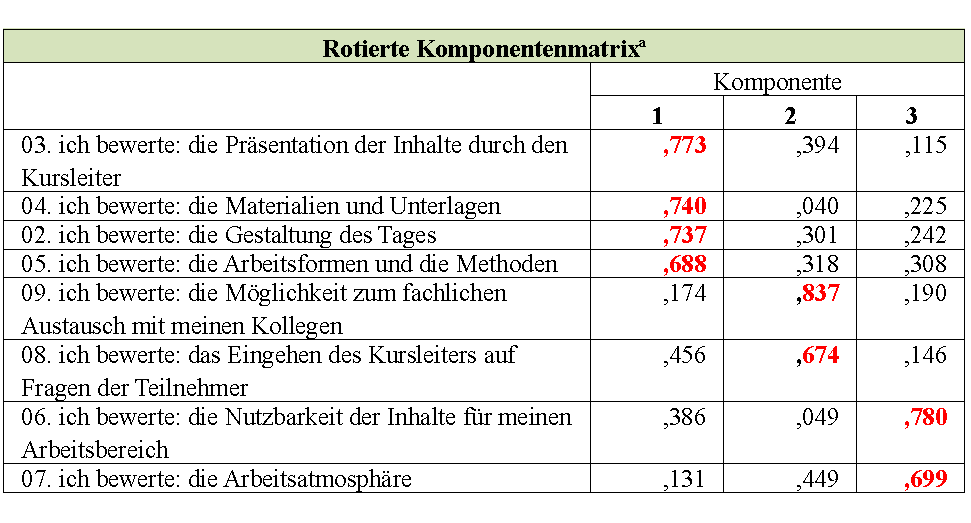
\includegraphics[scale=0.84]{tab7.pdf}
\caption{Rotierte Komponentenmatrix}
\label{tab3}
\end{table}
\FloatBarrier

Die einzelnen Items konnten in drei Kategorien zusammengefasst werden. 	
Der erste Faktor \textbf{"`Arbeitsformen"'} umfasst "`Präsentation der Inhalte durch den Kursleiter"', "`die Gestaltung des Tages"', "`die Materialien und Unterlagen"' sowie "`die Arbeitsformen und Methoden"', die im Kurs angewandt wurden.

Zum zweiten Faktor \textbf{"`fachlicher Austausch"'} gehören "`die Möglichkeit zum fachlichen Austausch mit den Kollegen"' im Kurs und "`das Eingehen des Kursleiters auf Fragen der Teilnehmer"'.

Der dritte Faktor \textbf{"`Arbeitsatmosphäre"' }beinhaltet folgende Items: "`die Nutzbarkeit der Inhalte für meinen Arbeitsbereich"' und "`die Ar\-beits\-at\-mos\-phä\-re"'.

\subsubsection{Regressionsanalyse}

Der Grundgedanke einer Regression liegt darin, die abhängige Variable aus der Kombination verschiedener unabhängiger Variablen vorherzusagen bzw. zu erklären. Mit Hilfe einer Regressionsgleichung können dann Aussagen darüber getroffen werden, welchen Einfluss die verschiedenen unabhängigen Variablen auf die abhängige Variable haben (vgl. Eid/Gollwitzer/Schmitt, 2010, S. 602-603). 

Die empirische Forschung unterscheidet zwischen verschiedenen Arten der Regressionsanalyse. Da in der vorliegenden Arbeit der Einfluss und die Art des Zusammenhangs von mehreren Prädiktoren \textit{("`die Bewertung der Gestaltung des Tages"', "`die Präsentation der Inhalte durch den Kursleiter"', "`Materialien und Unterlagen, Arbeitsformen und Methoden"', "`Nutzbarkeit der Inhalte für den eigenen Arbeitsbereich"', "`Arbeitsatmosphäre"', "`das Eingehen des Kursleiters auf Fragen der Teilnehmer"', "`die Möglichkeit zum fachlichen Austausch"', "`Erfahrungen als Kursleiter"' sowie "`das Alter"' und "`Geschlecht"')} auf die abhängige Variable \textit{"`Bewertung des Arbeitskreises insgesamt"'} überprüft werden soll, wird als Analyseverfahren die \textit{multiple Regression} gewählt. Mit ihr sollen Aussagen darüber getroffen werden, welche unabhängigen Variablen am stärksten die abhängige Variable vorhersagen.


\begin{table}[!ht]
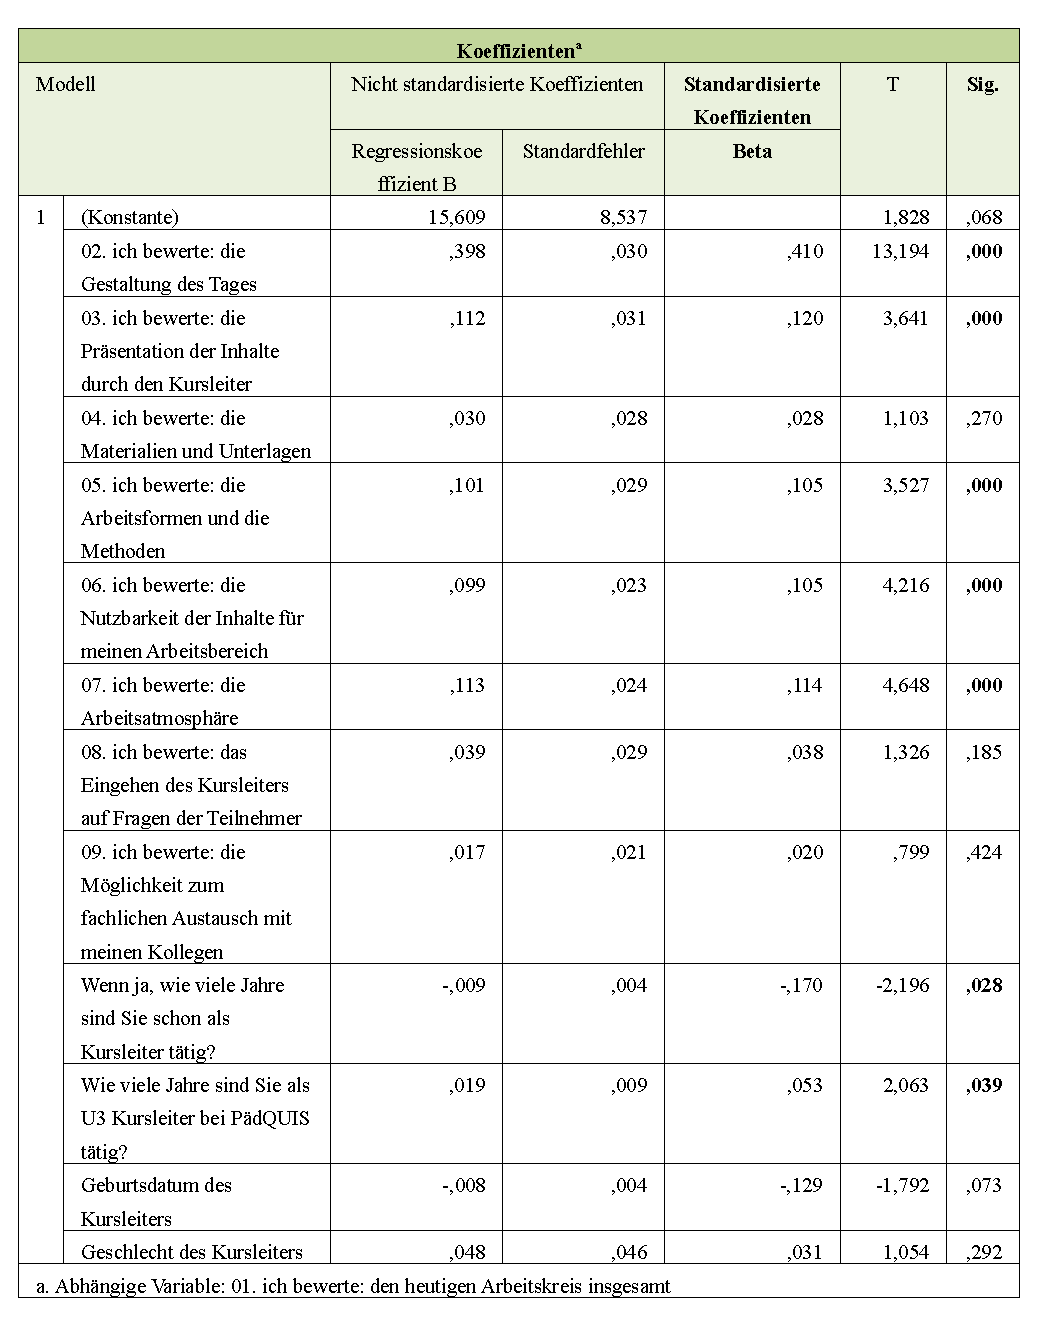
\includegraphics[scale=0.8]{tab08.pdf}
\caption{Regressionskoeffizienten}
\label{tab.4}
\end{table}
\FloatBarrier

Die Regressionsanalyse zeigt, dass 59,5\% der Gesamtvarianz durch die unabhängigen Variablen aufgeklärt ist. Aus der oben stehenden Tabelle geht hervor, dass die Variable \textit{"`Gestaltung des Tages"'} den stärksten Prädiktor für die Variable \textit{"`Bewertung des Arbeitskreises insgesamt"'} darstellt und sie somit am stärksten vorhersagt. Die Variable \textit{"`Erfahrung als Kursleiter"'} ist der zweithöchste Prädiktor. Am dritten Platz steht das Item \textit{"`Präsentation der Inhalte durch den Kursleiter"'}, gefolgt von Prädiktoren \textit{"`Arbeitsatmosphäre"'},  \textit{"`Arbeitsformen und Methoden"'} sowie \textit{"`Nutzbarkeit der Inhalte für eigenen Arbeitsbereich"'}. Ebenfalls als signifikant aus regressionsanalytischer Sicht hat sich auch der Aspekt \textit{"`Dauer der Tätigkeit als U3-Kursleiter bei PädQUIS"'} erwiesen. 

Alle anderen Prädiktoren haben zwar keinen signifikanten Einfluss auf die abhängige Variable, sind jedoch für die Zielvariable insofern nicht ohne Bedeutung, weil sie miteinander korrelieren. Dadurch werden unerwünschte Kollinearitäten erzeugt, was wiederum die Schätzung der Regressionsgleichung beeinträchtigen kann und bei den Regressionskoeffizienten zu verzerrten Resultaten führt. 

Zusammenfassend kann festgehalten werden, dass \textit{"`die Gestaltung des Tages"'} den stärksten Einfluss auf \textit{"`die Bewertung des Arbeitskreises insgesamt"'} hat, gefolgt von der Variable \textit{"`Erfahrung als Kursleiter"'}. Der dritte Stellenwert kommt der \textit{"`Präsentation der Inhalte durch den Kursleiter"'}, \textit{"`der Arbeitsatmosphäre"'},  \textit{"`den Arbeitsformen und Methoden"'} sowie \textit{"`der Nutzbarkeit der Inhalte für eigenen Arbeitsbereich"'} zu. 

\subsubsection{Multivariate Varianzanalyse}

Im nächsten Schritt wird \textit{multivariate Varianzanalyse} durchgeführt. Die Varianzanalyse ist eine Erweiterung des t-Tests. Der t-Test vergleicht zwei Mittelwerte miteinander. Wenn jedoch mehr als zwei Mittelwerte miteinander verglichen werden sollen, ist der t-Test dafür nicht ausreichend geeignet. Stattdessen wird in der Regel eine Varianzanalyse durchgeführt (vgl. Luhmann, 2010, S. 192).


In der vorliegenden Studie stammen die zu vergleichenden Mittelwerte aus unabhängigen Stichproben. Daher wird eine Varianzanalyse ohne Messwiederholung durchgeführt. Es wurde überprüft, wie und ob sich die sechs Kurs\-lei\-ter/-innen in ihren mittleren Werten in Bezug auf die drei errechneten Faktoren "`Arbeitsform"', "`Arbeitsatmosphäre"' und "`fachlichen Austausch"' voneinander unterscheiden. Eine wichtige Voraussetzung für die zu diesem Zweck durchgeführte multivariate Varianzanalyse ist die Varianzhomogenität, d. h. die Varianz der abhängigen Variablen in der Population sollte in allen Gruppen gleich sein. Es ist wichtig, diese Annahme zu überprüfen, bevor man eine Varianzanalyse durchführt. Diese Annahme kann zum Beispiel mit Hilfe von Levene-Test geprüft werden. Liegt Varianzhomogenität vor, sind die Varianzen also in allen Gruppen gleich. Ein signifikantes Ergebnis bedeutet dagegen, dass Varianzheterogenität vorliegt. In der vorliegenden Arbeit zeigt der Test einen signifikanten Wert von (p$<$ .05), d. h. die Nullhypothese der Varianzhomogenität wird verworfen. 
Dies wird in Tabelle 5 dargestellt.

%Levene-Test auf Gleichheit der Fehlervarianzena


\begin{table}
\begin{center}
\begin{tabular}{|l|r|r|r|r|}
\hline 
 & F & df1 & df2 & Sig. \\ 
\hline 
MW-Arbeitsform & 2.374 & 5 & 1005 & ,037 \\ 
\hline 
MW-Arbeitsatmosphäre & 5,894 & 5 & 1005 & ,000 \\ 
\hline 
MW-fach-Austausch & 8,002 & 5 & 1005 & ,000 \\ 
\hline 
\end{tabular} 
\end{center}
\caption{Levene-Test auf Gleichheit der Fehlervarianzen}
\end{table}
\FloatBarrier

Demzufolge liegen signifikante Mittelwertunterschiede zwischen den Kurs\-lei\-ter/-in\-nen hinsichtlich \textit{der Arbeitsform}, \textit{Arbeitsatmosphäre} und \textit{des fachlichen Austausches im Kurs} vor. Es ist jedoch erst mal nicht bekannt, welche Mittelwerte das sind. Dies lässt sich durch  \textit{das Post-hoc-Verfahren} bzw. den \textit{Duncan-Test} feststellen.


\begin{table}[!ht]
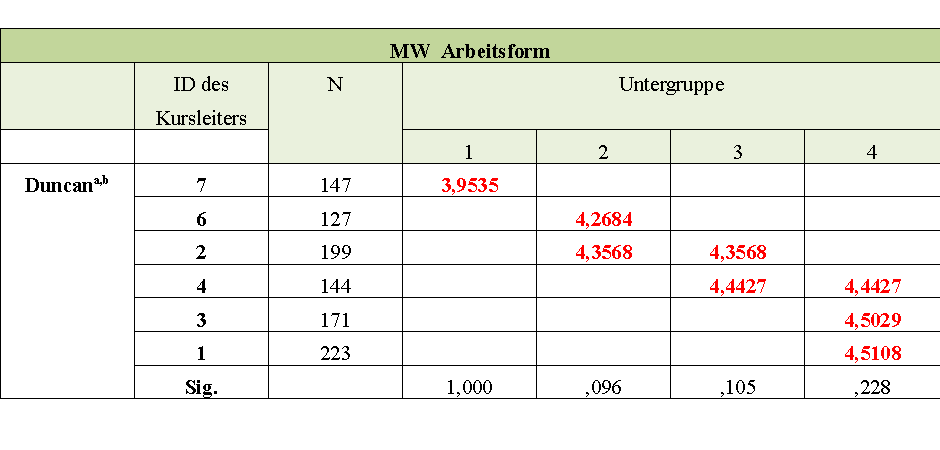
\includegraphics[scale=0.85]{tab01.pdf}
\caption{MW Arbeitsform}
\label{tab.6}
\end{table}
\FloatBarrier

Hinsichtlich \textit{der Arbeitsform} zeigen sich keine signifikanten Differenzen zwischen den Mittelwerten der Kursleiter/-innen \textbf{kl\_1, kl\_3} und \textbf{kl\_4}. Auch die Mittelwerte von \textbf{kl\_2} und \textbf{kl\_6} unterscheiden sich nicht signifikant von\-ei\-nan\-der. Der/die Kursleiter/-in \textbf{kl\_7} weist den niedrigsten Mittelwert im Vergleich zu den anderen Kursleitern auf. 

Es wurden keine signifikanten Unterschiede bezüglich \textit{der Arbeitsatmosphäre} zwischen den \textbf{kl\_1, kl\_3, kl\_2, kl\_4} und \textbf{kl\_6} festgestellt. Allerdings kann ein signifikanter Unterschied von \textbf{kl\_7} zu den anderen Kursleitern aufgezeigt werden. 


\begin{table}[!ht]
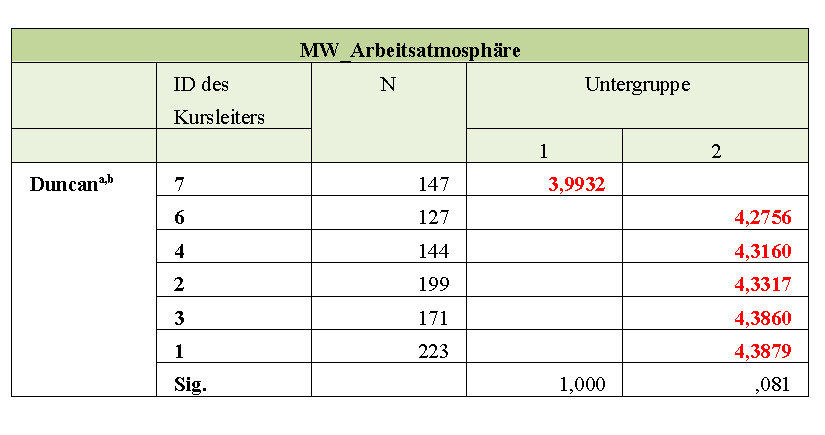
\includegraphics[scale=1.0]{tab02.pdf}
\caption{MW Arbeitsatmosphäre}
\label{tab.7}
\end{table}
\FloatBarrier


Die Tabelle 8 veranschaulicht, dass es sich kein signifikanter Unterschied zwischen den Mittelwerten von \textbf{kl\_1} und \textbf{kl\_3} sowie zwischen den \textbf{kl\_4} und \textbf{kl\_6} zeigt. Der Mittelwert von \textbf{kl\_7} unterscheidet sich wie auch bei \textit{der Arbeitsatmosphäre} und \textit{Arbeitsform} signifikant von den anderen Mittelwerten.

\begin{table}[!ht]
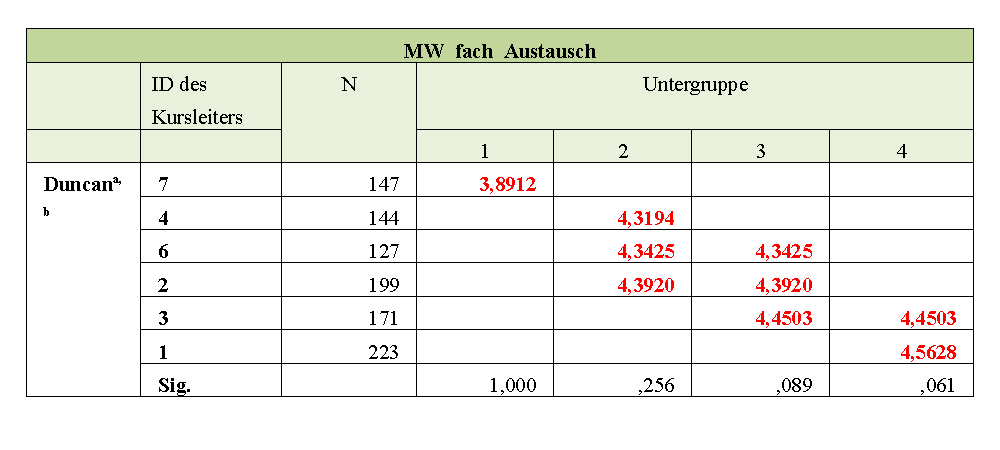
\includegraphics[scale=0.82]{tab03.pdf}
\caption{MW fachlicher Austausch}
\label{tab.8}
\end{table}
\FloatBarrier

Die durchgeführte Analyse hat ergeben, dass die Kursleiter/-innen \textbf{kl\_1} und \textbf{kl\_3} bei allen Kategorien am besten abschneiden, gefolgt von \textbf{kl\_2, kl\_4} und \textbf{kl\_6}. Die niedrigsten Werte bei allen drei Kategorien zeigt der/die \textbf{kl\_7}.

\subsubsection{Ergebnisse der Auswertung der offenen Fragen aus der Teilnehmerbefragung}

In der vorliegenden Arbeit erfolgte die Auswertung der offenen Fragen über ein quantitatives Auszählen der Antworten. Zunächst wurden die offenen Fragen des Teilnehmerfragebogens analysiert, um dann im nächsten Schritt darauf aufbauend ein Kategoriensystem zu entwickeln. Die Kategorienbildung bzw. die Kategorienformulierung orientierte sich an den Antworten der Teilnehmer/-innen. Wenn zu der Frage\textit{ "`Gut gefallen hat mir heute…"'} beispielsweise verschiedene Arbeitsformen  genannt wurden, so wurden diese der Kategorie \textit{"`Methoden"'} zugeordnet. Die ausführliche Darstellung des Kategorienmodells ist dem Anhang beigefügt.

Die Tabelle 9 enthält eine Übersicht über die Häufigkeiten der Antworten der Teilnehmer/-innen auf die offenen Fragen. Wie bereits oben ausgeführt, haben wir die gesamten Antworten zum Zweck der besseren Datenhandhabung und besseren Ü\-ber\-blicks zu Kategorien (siehe obere Zeile der Tabelle) zusammengefasst. Dabei ergab die Auswertung folgende Ergebnisse: einen großen Wert legen die Teil\-neh\-mer/-in\-nen auf ausreichend vielfältige Methoden- und Fachkenntnisse bzw. Qualifikationen der Referenten/-innen. So wurde auf die Frage\textit{ "`Gut gefallen hat mir heute…"'} 136 Mal die Kategorie \textit{"`Dozent"'} sowie die Kategorie \textit{"`Input/Anregungen"'} angegeben. Unter anderem haben die Teilnehmer/-innen folgende Eigenschaften der Dozenten hervorgehoben: 

\textit{"`Motivation und Freude der Moderatorin"'},
\textit{"`Die Art und Weise von X, kompetent, nicht langsam, nicht gewollt komisch aber locker mit Humor"'}.

	Am häufigsten kommt in den Antworten der Teilnehmenden die Kategorie \textit{"`Methoden"'} vor. Diese Kategorie wurde auf die Frage \textit{"`Gut gefallen hat mir…"'} 805 Mal angegeben. Im negativen Kontext auf die Frage \textit{"`Nicht gefallen hat mir…"'} wurde sie lediglich 174 Mal genannt. In der Kategorie \textit{"`Methoden"'} waren häufig genannte Aspekte vor allem: 
	
\textit{ "`Die Methodenvielfalt"'},
\textit{"`Die Kleingruppenarbeit, dadurch ergab sich ein guter Austausch mit den Kollegen. [Wunsch]Häufiger Kleingruppenarbeit"'}.

Des Weiteren wurden häufig der kollegiale Austausch, das Arbeitsmaterial, die im Kurs behandelten Themenbereiche sowie praxisorientierte Inhalte genannt.

Bei der Frage \textit{"`Nicht gefallen hat mir heute"'} stellt neben der Kategorie \textit{"`Methoden"' }(174 Nennungen)\textit{ "`die Erfüllung der Grundbedürfnisse"'} mit 62 Nennungen (z.B. Raumgestaltung/-klima, Verpflegung) sowie \textit{"`die Zeiteinteilung"'} mit 54 Nennungen einen wichtigen Aspekt dar. Folglich spielen für die Zufriedenheitsbewertung des Kurses sowohl die Erfüllung der Grundbedürfnisse als auch der Zeitmanagement eine wesentliche Rolle. 

Die Frage \textit{"`Wenn Sie für Aspekte die Bewertung "`weniger gut"' oder "`gar nicht gut"' vergeben haben, was waren die Gründe für Ihre Entscheidung?"'} wurde nur selten beantwortet. Mit 26 Nennungen wurde auf diese Frage die Kategorie \textit{"`kollegialer Austausch"'} am häufigsten genannt:

\textit{ "Mehr Austausch mit den Kolleginnen fände ich wünschenswert"'},
\textit{ "Der gegenseitige Austausch kommt öfters etwas zu kurz"'}.

Basierend auf den Antworten auf die letzte Frage \textit{"`Ein Abschlusssatz von Ihnen zum heutigen Arbeitskreis für uns zum Mitnehmen"'} kann ein Schluss gezogen werden, dass das Qualifizierungsprogramm für die pädagogischen Fachkräfte eine gute Anregung für die Arbeit mit Kindern unter drei Jahren darstellt. Die Kategorie \textit{"`Die Motivation zur weiteren Teilnahme/Arbeit mit U3 Kindern"'} weist hier mit 808 Nennungen den höchsten Wert auf. Auch \textit{"`die praxisorientierten Inhalte"'} (126 Nennungen) sowie \textit{"`die Methoden"'} (128 Nennungen) spielen für die Teilnehmer/-innen eine wichtige Rolle. 
\begin{center}
\begin{table}[!ht]
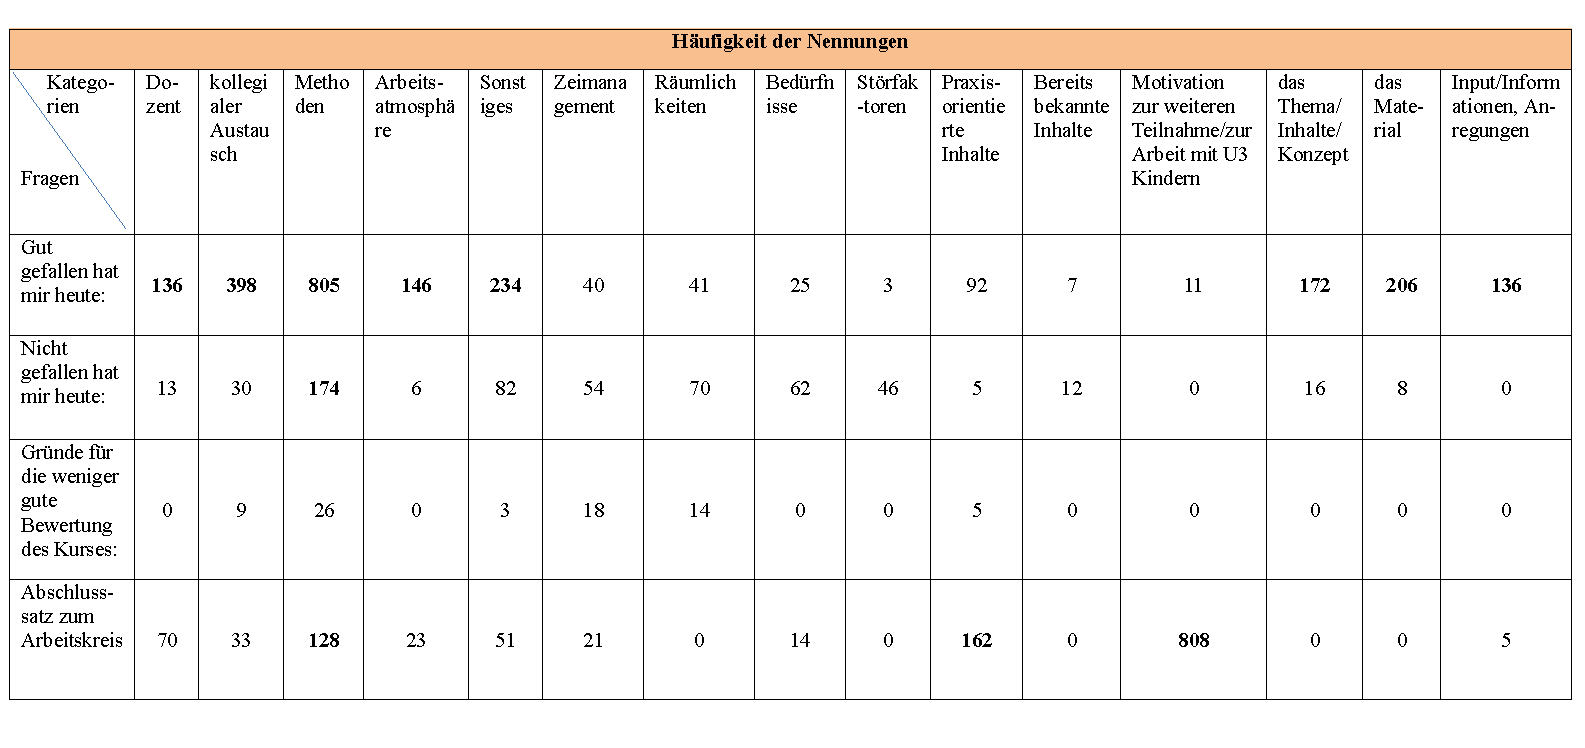
\includegraphics[scale=0.71,angle=90]{tab04.pdf}
\caption{Häufigkeiten der offenen Fragen}
\label{tab.9}
\end{table}
\end{center}



\section{Zusammenfassung der Ergebnisse und Diskussion}

Das Ziel dieses Projektes war es, den Lesern einen Einblick in die Weiterbildungsthematik anhand der Ergebnisse der aktuellen Forschung zu er\-mög\-li\-chen sowie das Fortbildungs- und Qualifizierungsprogramm zur Betreuung, Bildung und Erziehung von Kindern unter drei Jahren \textit{"`Qualität von Anfang an"'} exemplarisch vorzustellen und zu analysieren. 
Im Hinblick auf die Forschungsfrage werden in diesem Abschnitt anhand von gewonnenen Ergebnissen Schluss\-folgerungen gezogen. Unsere Forschungsfrage lautete: 

\textit{Wodurch zeichnet sich gute Qualität im Programm zur Betreuung, Bildung und Erziehung von Kindern unter drei Jahren \textit{"`Qualität von Anfang an"'} aus und durch welche Faktoren wird sie beeinflusst?}

Der Einblick in die Weiterbildungslandschaft macht deutlich, dass die Fort- und Weiterbildung in unserer Gesellschaft immer mehr an Bedeutung gewinnt. Sowohl die gestiegenen Qualifikationsanforderungen als auch der Qualifikationserhalt sind hierfür wesentliche Aspekte. Die Existenzsicherung hängt heutzutage im besonders starken Maße von den erworbenen Qualifikationen ab. Aufgabe der Weiterbildung ist es daher, die Diskrepanz zwischen neuen Anforderungen des Arbeitsplatzes und den vorhandenen Qualifikationen durch Fortbildungsangebote abzubauen.

Durch den gesellschaftlichen Wandel und die Bildungsdebatte rückt auch die Fort- und Weiterbildung frühpädagogischer Fachkräfte in den Fokus der Öffentlichkeit. Insbesondere steht dabei die Qualifizierung der Erzieher/-innen im Zentrum der Diskussion. Die pädagogischen Fachkräfte werden gegenwärtig und zukünftig vor neue Anforderungen gestellt. Der quantitative Ausbau von Angeboten der Betreuung, Bildung und Erziehung, beispielsweise die Realisierung des Rechtsanspruchs auf einen Kindergartenplatz ab drei Jahren, die Notwendigkeit eines pädagogischen Konzepts sowie die Einführung länderspezifischer Bildungsprogramme und –pläne stellen dabei die größten Herausforderungen dar. Die Grundausbildung der pädagogischen Fachkräfte legt das Fundament für die Professionalisierung, bedeutet aber nicht das Ende, sondern eher den Anfang der beruflichen Qualifizierung. 

Mit dem Anstieg des Qualifizierungsbedarfs stieg auch die Anzahl der Fort- und Weiterbildungsangebote für frühpädagogische Fachkräfte. Diese sind jedoch undurchschaubar und von unterschiedlicher Qualität. Folglich sind sie sowohl für die Adressaten als auch für die Anbieter schwer zu über\-bli\-cken und einzuschätzen. Um mehr Transparenz und Vergleichbarkeit auf dem Weiterbildungsmarkt zu schaffen, wurden durch eine Expertengruppe einheitliche Qualitätsstandards für die Fort- und Weiterbildung der früh\-pä\-da\-gogi\-schen Fachkräfte formuliert. Die Qualitätsstandards werden nach Orientierungs-, Struktur-, Prozess- und Ergebnisqualität differenziert. Aus den Leitlinien respektive Qualitäts\-stan\-dards geht hervor, dass die Zufriedenheitsbewertung des Kurses durch die Teilnehmenden ein wesentliches Kriterium für die Qualität der Fort- und Weiterbildung darstellt. Die Zufriedenheit der Teilnehmer/-innen bildet auch in der vorliegenden Studie einen zentralen Qualitätsstandard. Sie gibt Auskunft über den Erfolg des Programms, aber auch Hinweise auf Stärken und Schwächen der Angebote.

Die Zufriedenheitsbewertung der Teilnehmer/-innen spielt auch im Programm \textit{"`Qualität von Anfang an"' }eine wichtige Rolle. Durch die durchgeführte Analyse des Programms können die Adressaten einen guten Über\-blick über das Programm, die angebotenen Themen und deren Inhalte, Arbeitsformen und –materialien, die Qualifizierung der Referent/-innen sowie über den Weiterbildungsanbieter erhalten. Die Untersuchung gibt einerseits Auskunft darüber, inwieweit das Programm \textit{"`Qualität von Anfang an"'} ein attraktives Bildungsangebot für die frühpädagogischen Fachkräfte darstellt und deren Bedürfnissen sowie Erwartungen entspricht. Andererseits informiert sie auch den Anbieter über die Erfolge bzw. die Verbesserungsvorschläge/-bedarf in der weiteren Entwicklung des Programms.

Abschließend folgt eine kurze Zusammenfassung der Ergebnisse unserer empirischen Untersuchung. Zur Auswertung der Daten wurden die deskriptiven Maße, Faktoren- und multiple Regressionsanalyse sowie multivariate Varianzanalyse angewandt. Die Ergebnisse zeigen, dass die Teilnehmer/-innen insgesamt mit dem Programm zufrieden sind. Die Bewertung liegt im Durchschnitt bei einer Beurteilung "`gut"' bis "`sehr gut"'. Der höchste Mittelwert mit $\bar x$= 4,53 wurde beim Item\textit{ "`Eingehen des Kursleiters auf Fragen der Teilnehmer"' }ermittelt. Den niedrigsten Mittelwert mit $\bar x$= 4,18 weist der Aspekt \textit{"`Die Möglichkeit zum fachlichen Austausch mit Kollegen"'} auf. Insgesamt unterscheiden sich die Mittelwerte der Items nur marginal voneinander. 
Weiterhin hat die Analyse ergeben, dass der fachlich-kollegiale Austausch mit den Kollegen sowie die Praxisnähe des Kurses eine wesentliche Rolle für die Zufriedenheit mit dem Kurs spielen. 

Die weitere Untersuchung ergab, dass eine große Bedeutung bei der Beurteilung der Zufriedenheit von Teilnehmer/-innen mit dem jeweiligen Arbeitskreis den Prädiktoren \textit{"`Gestaltung des Tages"'}, \textit{"`Kursleitererfahrungen"'}, \textit{"`Präsentation der Inhalte durch den/die Kursleiter/-in"', "`Ar\-beits\-at\-mos\-phä\-re"', "`Arbeitsform und Methoden"', "`Nutzbarkeit der Inhalte für eigenen Arbeitsbereich"'} sowie \textit{"`Kursleitertätigkeit im Themenbereich U3"'} zukommt. Die Variable \textit{"`Gestaltung des Tages"'} sagte dabei am stärksten die Variable \textit{"`Bewertung des Arbeitskreises insgesamt"'} vorher. Keinen signifikanten Einfluss haben das Alter und das Geschlecht der Kursleiter/-innen, Materialien und Unterlagen, das Eingehen des Kursleiters auf die Fragen der Teilnehmer/-innen sowie die Möglichkeit zum fachlichen Austausch mit eigenen Kollegen auf die Bewertung des Arbeitskreises insgesamt. Das bedeutet jedoch nicht, dass diese Faktoren gar keinen Einfluss auf \textit{"`die Bewertung des Arbeitskreises insgesamt"'} ausüben.

Aufgrund der durchgeführten Analyse lassen sich die zuvor aufgestellten Hypothesen:

\textit{"`Je besser die Bewertung der Gestaltung des Tages, desto besser die Bewertung des Arbeitskreises insgesamt"'},
 
\textit{"`Je besser die Bewertung der Präsentation der Inhalte durch den Kursleiter, desto besser die Bewertung des Arbeitskreises insgesamt"'},

\textit{"`Je besser die Bewertung der Arbeitsform und Methoden, desto besser die Bewertung des Arbeitskreises insgesamt"',}

\textit{"`Je besser die Bewertung der Nutzbarkeit der Inhalte für den eigenen Arbeitsbereich, desto besser die Bewertung des Arbeitskreises insgesamt"'}
sowie die Hypothese \textit{"`Je besser die Bewertung Arbeitsatmosphäre, desto besser die Bewertung des Arbeitskreises insgesamt"'} bestätigen.

Überraschenderweise wurde die Hypothese \textit{"`Je mehr Erfahrung die Re\-fe\-renten/-innen als Kursleiter haben, desto besser fällt die Beurteilung des Kurses durch die Teilnehmer/-innen aus"'} durch die Ergebnisse widerlegt. Die Auswertung der Daten hat gezeigt, dass die  Dauer der Kursleitererfahrung nicht zwangsläufig mit einer positiven Bewertung des Kurses zusammenhängt. Im Gegenteil wurde im Rahmen unserer Studie die Qualität der Kurse von Kursleitern mit weniger Erfahrung von Teilnehmenden tendenziell besser bewertet. Die Gründe dafür können sehr vielfältig sein. Es wäre interessant, diese genauer zu untersuchen. An dieser Stelle können nur Annahmen gemacht werden. Beispielsweise könnte dieses Ergebnis darauf zurückzuführen sein, dass die Kursleiter mit mehr Erfahrung routinierter in ihrem Vorgehen sind und daher vielleicht weniger Bereitschaft zeigen, innovative Methoden einzusetzen. Während die Einsteiger/-innen häufig "`frischen Wind"' mitbringen, was ihre Veranstaltungen interessanter und anregender macht.

Weitere interessante Ergebnisse ergab die multivariate Varianzanalyse. In den vorgenommenen Vergleichen zwischen den Gruppen wird deutlich, dass sich die sechs Kursleiter/-innen in ihren mittleren Werten in Bezug auf die drei errechneten Faktoren \textit{"`Arbeitsform"'}, \textit{"`Arbeitsatmosphäre"'} und \textit{"`fachlichen Austausch"'} voneinander unterscheiden. Die Differenzen sind jedoch nicht signifikant. Die Abweichungen sind minimal, sodass keine bedeutenden Unterschiede zu verzeichnen sind. Lediglich bei einem Kursleiter konnte ein signifikanter Unterschied zu den Anderen aufgezeigt werden. Die Bewertung des Kurses von kl\_7 liegt im Bereich von "`teilweise gut"' bis "`gut"', während die Veranstaltungen aller anderen Kursleiter/-innen  mit "`gut"' bis "`sehr gut"' bewertet wurden. Auch in diesem Fall können wir nur Vermutungen anstellen, denn der Grund für diese Differenz vielfältige Ursachen haben könnte. Die Aufklärung dieser Varianz war mit den vorliegenden Daten aus den Kursleiterfragebögen nicht möglich. Um eine eindeutige Aussage treffen zu können, müssten noch weitere Daten erhoben werden. Somit konnte die Hypothese \textit{"`Je mehr Erfahrung die Referenten als Kursleiter/-innen haben, desto besser fällt die Beurteilung des Kurses durch die Teilnehmer/-innen aus"'} nicht verifiziert werden.

Die Auswertung der offenen Fragen untermauern die Ergebnisse der quantitativen Analyse. So spielen auch hier die Fachkenntnisse beziehungsweise die Qualifikation der Referenten, ausreichend vielfältige Methoden, kollegialer Austausch, Arbeitsmaterial, Themenbereiche sowie praxisorientierte Inhalte eine wichtige Rolle für die Bewertung der Zufriedenheit mit dem Programm. Eine sehr positive Auswertung der Kategorie\textit{ "`Motivation zur weiteren Teilnahme/Arbeit mit U3 Kindern"'} zeugt ebenfalls von einer hohen Zufriedenheit der Teilnehmer/-innen mit\textit{ "`Qualität von Anfang an"'}. Diese Kategorie weist mit 808 Nennungen die größte Häufigkeit auf. Wichtig für die Teilnehmer/-innen ist außerdem die Zufriedenstellung der Grundbedürfnisse. So bestimmen die Faktoren wie Raumklima, -gestaltung, Verpflegung sowie Zeitmanagement neben den didaktischen Aspekten die Gesamtbewertung des Kurses wesentlich mit. 

Zusammenfassend lässt sich sagen, dass die Zufriedenheit mit\textit{ "`Qualität von Anfang an"'}  bemerkenswert hoch ausfällt, was für eine gute Qualität des Programms spricht. Neben hoher Zufriedenheit erfüllt das Programm besonders zufriedenstellend weitere durch die Experten aufgestellte Qualitätsstandards, wie beispielsweise die Praxisorientierung der Inhalte und die Qualifizierung der Referenten. 

Abschließend lässt sich sagen, dass das Programm \textit{"`Qualität von Anfang an"'} den wesentlichen Qualitätskriterien entspricht. Es stellt ein attraktives Fortbildungsangebot für frühpädagogische Fachkräfte dar und erfüllt deren Bedürfnisse und Erwartungen. 
Wichtig ist dabei hinzuweisen, dass für die Beurteilung der Qualität eines Programms, die reine Zufriedenheitsabfrage jedoch nicht ausreicht. Um Qualität der Fort- und Weiterbildung möglichst objektiv und umfassend erfassen zu können, bedarf es weiterer Maßnahmen wie beispielsweise Outputevaluationen oder Lerntransfererhebungen. Das sollte im nächsten Forschungsschritt  geschehen. 



\pagebreak

\bibliographystyle{alphadin} 
\bibliography{Forschungsbericht}
\section*{Literaturverzeichnis}
\addcontentsline{toc}{section}{Literaturverzeichnis}

Arbeitsgruppe Bildungsbericht am Max-Planck-Institut für Bildungsforschung (1994). Das Bildungswesen in der Bundesrepublik Deutschland. Strukturen und Entwicklungen im Überblick. Hamburg.\\

Autorengruppe Bildungsberichterstattung (2010). 
Bildung in Deutschland 2010. Ein Indikatoren gestützter Bericht mit einer Analyse zu Perspektiven des Bildungswesens im demografischen Wandel. Im Auftrag der Ständigen Konferenz der Kultusminister der Länder in der Bundesrepublik Deutschland und des Bundesministeriums für Bildung und Forschung. Bielefeld.\\

Autorengruppe Bildungsberichterstattung (2012) (Hrsg.). Bildung in Deu\-tsch\-land 2012: Ein indikatorengestützter Bericht mit einer Analyse zur kulturellen Bildung im Lebenslauf.
URL: \url{http://www.bildungsbericht.de/daten2012/bb_2012.pdf}(Zugriff am 20.03.2013).\\

Baumeister, K., \& Grieser, A. (2011). Berufsbegleitende Fort- und Weiterbildung frühpädagogischer Fachkräfte - Analyse der Programmangebote. Weiterbildungsintiative Frühpädagogischer Fachkräfte, Erziehungswissenschaften. München: Deutsches Jugendinstitut e.V.\\

Bühl, A. (2006). SPSS 14. Einführung in die moderne Datenanalyse. München: Pearson Studium.\\

Dittrich, I.,Grenner, K., Groot-Wilken, B., Sommerfeld, V., Hanisch, A. (2007).Pädagogische Qualität in Tageseinrichtungen für Kinder.Ein nationaler Kriterienkatalog . Tietze,W.,Viernickel,S.(Hrsg.).3. Aufl.,Berlin, Düsseldorf, Mannheim: Cornelsen Verlag.\\

Eid/Gollwitzer/Schmitt (2010). Statistik und Forschungsmethoden. Weinheim, Basel: Beltz.\\

Expertengruppe Berufsbegleitende Weiterbildung (2011). Qualität in der Fort- und Weiterbildung von pädagogischen Fachkräften in Kindertageseinrichtungen – Standards für Anbieter. München. Deutsches Jugendinstitut e.V.\\ 

Faulstich, P. (1993). "`Mittlere Systematisierung"' der Weiterbildung, in: Meier, A. \& Rabe-Kleberg, U. (Hrsg.). Weiterbildung, Lebenslauf, sozialer Wandel, Reihe. Grundlage der Weiterbildung. Neuwied, Kriftel, Berlin, S. 29-46\\
Görs, D., \& Schlaffke, W. (1982). Die gesellschaftspolitische Bedeutung der Weiterbildung - aus der Sicht der Unternehmen und der Arbeitnehmer (Bd. 23). (J. Münch, Hrsg.) Berlin: Erich Schmidt Verlag GmbH.\\

Hippel, A., \& Grimm, R. (2010). Qualitätsentwicklungskonzepte in der Weiterbildung frühpädagogischer Fachkräfte. (D. J. e.V., Hrsg.). URL: http://\-www.wei\-ter\-bil\-dungs\-ini\-tia\-tive.de (Zugriff am 28. März 2013).\\

Kirchhöfer, Dieter (2004): Lernkultur Kompetenzentwicklung Begriffliche Grundlagen. Berlin. \\

Krenz, Armin (2001): Qualitätssicherung in Kindertagesstätten. Kieler Instrumentarium für Elementarpädagogik und Leistungsqualität. K.I.E.L. München. München.\\

Lasson, A., \& Grenner, K. (1. Januar 2008). Krippenkinder - Herausforderung und Chance für die berufliche Ausbildung. Klein und Groß , S. 45-49.\\

"Lernen bedeutet leben". URL: http://www.lernen-bedeutet-leben.de/news\-/items/persoenliche-zufriedenheit-durch-berufliche-weiterbildung (Zugriff am 6.04.2013).\\

Luhmann, M. (2010). R für Einsteiger. Einführung in die Statistiksoftware für die Sozialwissenschaften. Beltz: Weinheim, Basel.\\

Mangold, M., Casper, S., \& Hochmuth, U. (1996). Qualifizierung im Strukturwandel: Zur Bedeutung der Weiterbildung (Bd. 15). Tübingen, Basel: Francke.\\

OECD (2004). Die Politik der frühkindlichen Betreuung, Bildung und Erziehung in der Bundesrepublik Deutschland Ein Länderbericht der Organisation für wirtschaftliche Zusammenarbeit und Entwicklung (OECD). Bundesministerium für Familie, Senioren, Frauen und Jugend. Berlin.\\

PädQUIS (2010). U3-Rahmenkonzeption.\\

Tietze, W., Meischner, T., Gänsfuß, R., Grenner, K., Schuster, K.-M., Völkel, P., et al. (1998). Wie gut sind unsere Kindergärten? Eine Untersuchung zur pädagogischen Qualität in deutschen Kindergärten. (W. Tietze, Hrsg.) Berlin: Luchterhand.



\pagebreak

\begin{appendix}
\section*{Anhang}
\addcontentsline{toc}{section}{Anhang}
\normalsize
\section{}
\end{appendix}
  
\end{document}